\documentclass[twoside]{book}

% Packages required by doxygen
\usepackage{fixltx2e}
\usepackage{calc}
\usepackage{doxygen}
\usepackage[export]{adjustbox} % also loads graphicx
\usepackage{graphicx}
\usepackage[utf8]{inputenc}
\usepackage{makeidx}
\usepackage{multicol}
\usepackage{multirow}
\PassOptionsToPackage{warn}{textcomp}
\usepackage{textcomp}
\usepackage[nointegrals]{wasysym}
\usepackage[table]{xcolor}

% Font selection
\usepackage[T1]{fontenc}
\usepackage[scaled=.90]{helvet}
\usepackage{courier}
\usepackage{amssymb}
\usepackage{sectsty}
\renewcommand{\familydefault}{\sfdefault}
\allsectionsfont{%
  \fontseries{bc}\selectfont%
  \color{darkgray}%
}
\renewcommand{\DoxyLabelFont}{%
  \fontseries{bc}\selectfont%
  \color{darkgray}%
}
\newcommand{\+}{\discretionary{\mbox{\scriptsize$\hookleftarrow$}}{}{}}

% Page & text layout
\usepackage{geometry}
\geometry{%
  a4paper,%
  top=2.5cm,%
  bottom=2.5cm,%
  left=2.5cm,%
  right=2.5cm%
}
\tolerance=750
\hfuzz=15pt
\hbadness=750
\setlength{\emergencystretch}{15pt}
\setlength{\parindent}{0cm}
\setlength{\parskip}{3ex plus 2ex minus 2ex}
\makeatletter
\renewcommand{\paragraph}{%
  \@startsection{paragraph}{4}{0ex}{-1.0ex}{1.0ex}{%
    \normalfont\normalsize\bfseries\SS@parafont%
  }%
}
\renewcommand{\subparagraph}{%
  \@startsection{subparagraph}{5}{0ex}{-1.0ex}{1.0ex}{%
    \normalfont\normalsize\bfseries\SS@subparafont%
  }%
}
\makeatother

% Headers & footers
\usepackage{fancyhdr}
\pagestyle{fancyplain}
\fancyhead[LE]{\fancyplain{}{\bfseries\thepage}}
\fancyhead[CE]{\fancyplain{}{}}
\fancyhead[RE]{\fancyplain{}{\bfseries\leftmark}}
\fancyhead[LO]{\fancyplain{}{\bfseries\rightmark}}
\fancyhead[CO]{\fancyplain{}{}}
\fancyhead[RO]{\fancyplain{}{\bfseries\thepage}}
\fancyfoot[LE]{\fancyplain{}{}}
\fancyfoot[CE]{\fancyplain{}{}}
\fancyfoot[RE]{\fancyplain{}{\bfseries\scriptsize Generated by Doxygen }}
\fancyfoot[LO]{\fancyplain{}{\bfseries\scriptsize Generated by Doxygen }}
\fancyfoot[CO]{\fancyplain{}{}}
\fancyfoot[RO]{\fancyplain{}{}}
\renewcommand{\footrulewidth}{0.4pt}
\renewcommand{\chaptermark}[1]{%
  \markboth{#1}{}%
}
\renewcommand{\sectionmark}[1]{%
  \markright{\thesection\ #1}%
}

% Indices & bibliography
\usepackage{natbib}
\usepackage[titles]{tocloft}
\setcounter{tocdepth}{3}
\setcounter{secnumdepth}{5}
\makeindex

% Hyperlinks (required, but should be loaded last)
\usepackage{ifpdf}
\ifpdf
  \usepackage[pdftex,pagebackref=true]{hyperref}
\else
  \usepackage[ps2pdf,pagebackref=true]{hyperref}
\fi
\hypersetup{%
  colorlinks=true,%
  linkcolor=blue,%
  citecolor=blue,%
  unicode%
}

% Custom commands
\newcommand{\clearemptydoublepage}{%
  \newpage{\pagestyle{empty}\cleardoublepage}%
}

\usepackage{caption}
\captionsetup{labelsep=space,justification=centering,font={bf},singlelinecheck=off,skip=4pt,position=top}

%===== C O N T E N T S =====

\begin{document}

% Titlepage & ToC
\hypersetup{pageanchor=false,
             bookmarksnumbered=true,
             pdfencoding=unicode
            }
\pagenumbering{alph}
\begin{titlepage}
\vspace*{7cm}
\begin{center}%
{\Large Tetris 2020 \\[1ex]\large 1.\+0 }\\
\vspace*{1cm}
{\large Generated by Doxygen 1.8.13}\\
\end{center}
\end{titlepage}
\clearemptydoublepage
\pagenumbering{roman}
\tableofcontents
\clearemptydoublepage
\pagenumbering{arabic}
\hypersetup{pageanchor=true}

%--- Begin generated contents ---
\chapter{Namespace Index}
\section{Namespace List}
Here is a list of all documented namespaces with brief descriptions\+:\begin{DoxyCompactList}
\item\contentsline{section}{\hyperlink{namespaceStates}{States} \\*Each view existing in game }{\pageref{namespaceStates}}{}
\end{DoxyCompactList}

\chapter{Hierarchical Index}
\section{Class Hierarchy}
This inheritance list is sorted roughly, but not completely, alphabetically\+:\begin{DoxyCompactList}
\item \contentsline{section}{Application}{\pageref{classApplication}}{}
\item \contentsline{section}{Client}{\pageref{classClient}}{}
\item \contentsline{section}{State\+:\+:Context}{\pageref{structState_1_1Context}}{}
\item Drawable\begin{DoxyCompactList}
\item \contentsline{section}{Component}{\pageref{classComponent}}{}
\begin{DoxyCompactList}
\item \contentsline{section}{Background}{\pageref{classBackground}}{}
\item \contentsline{section}{Button}{\pageref{classButton}}{}
\item \contentsline{section}{Grid}{\pageref{classGrid}}{}
\item \contentsline{section}{Label}{\pageref{classLabel}}{}
\end{DoxyCompactList}
\end{DoxyCompactList}
\item \contentsline{section}{Matrix}{\pageref{classMatrix}}{}
\item Non\+Copyable\begin{DoxyCompactList}
\item \contentsline{section}{Component}{\pageref{classComponent}}{}
\item \contentsline{section}{State\+Manager}{\pageref{classStateManager}}{}
\end{DoxyCompactList}
\item \contentsline{section}{Player}{\pageref{classPlayer}}{}
\item \contentsline{section}{State}{\pageref{classState}}{}
\begin{DoxyCompactList}
\item \contentsline{section}{Game\+Scene}{\pageref{classGameScene}}{}
\item \contentsline{section}{Help\+Scene}{\pageref{classHelpScene}}{}
\item \contentsline{section}{Menu\+Scene}{\pageref{classMenuScene}}{}
\item \contentsline{section}{Multiplayer\+Scene}{\pageref{classMultiplayerScene}}{}
\item \contentsline{section}{Pause\+Scene}{\pageref{classPauseScene}}{}
\item \contentsline{section}{Title\+Scene}{\pageref{classTitleScene}}{}
\end{DoxyCompactList}
\item \contentsline{section}{Tetromino}{\pageref{classTetromino}}{}
\item Transformable\begin{DoxyCompactList}
\item \contentsline{section}{Component}{\pageref{classComponent}}{}
\end{DoxyCompactList}
\item \contentsline{section}{Utility}{\pageref{classUtility}}{}
\end{DoxyCompactList}

\chapter{Class Index}
\section{Class List}
Here are the classes, structs, unions and interfaces with brief descriptions\+:\begin{DoxyCompactList}
\item\contentsline{section}{\hyperlink{classApplication}{Application} \\*Responsible for all initialization of the project }{\pageref{classApplication}}{}
\item\contentsline{section}{\hyperlink{classBackground}{Background} }{\pageref{classBackground}}{}
\item\contentsline{section}{\hyperlink{classButton}{Button} \\*Abstraction of a button component to implement in the view }{\pageref{classButton}}{}
\item\contentsline{section}{\hyperlink{classClient}{Client} }{\pageref{classClient}}{}
\item\contentsline{section}{\hyperlink{classComponent}{Component} \\*Mother class for the components created, which compiles S\+F\+ML functions }{\pageref{classComponent}}{}
\item\contentsline{section}{\hyperlink{structState_1_1Context}{State\+::\+Context} \\*Structure that references the current context screen }{\pageref{structState_1_1Context}}{}
\item\contentsline{section}{\hyperlink{classGameScene}{Game\+Scene} \\*Responsible for sampling the main screen of the singleplayer game }{\pageref{classGameScene}}{}
\item\contentsline{section}{\hyperlink{classGrid}{Grid} \\*Build the meshes responsible for making the tetris table }{\pageref{classGrid}}{}
\item\contentsline{section}{\hyperlink{classHelpScene}{Help\+Scene} \\*Responsible for viewing the help page of the game }{\pageref{classHelpScene}}{}
\item\contentsline{section}{\hyperlink{classLabel}{Label} \\*Compiles within itself the tools to create a label through S\+F\+ML }{\pageref{classLabel}}{}
\item\contentsline{section}{\hyperlink{classMatrix}{Matrix} }{\pageref{classMatrix}}{}
\item\contentsline{section}{\hyperlink{classMenuScene}{Menu\+Scene} \\*Responsible for viewing the game\textquotesingle{}s main menu }{\pageref{classMenuScene}}{}
\item\contentsline{section}{\hyperlink{classMultiplayerScene}{Multiplayer\+Scene} \\*Class responsible for taking care of the introduction Multiplayer screen of the game }{\pageref{classMultiplayerScene}}{}
\item\contentsline{section}{\hyperlink{classPauseScene}{Pause\+Scene} }{\pageref{classPauseScene}}{}
\item\contentsline{section}{\hyperlink{classPlayer}{Player} }{\pageref{classPlayer}}{}
\item\contentsline{section}{\hyperlink{classState}{State} }{\pageref{classState}}{}
\item\contentsline{section}{\hyperlink{classStateManager}{State\+Manager} }{\pageref{classStateManager}}{}
\item\contentsline{section}{\hyperlink{classTetromino}{Tetromino} }{\pageref{classTetromino}}{}
\item\contentsline{section}{\hyperlink{classTitleScene}{Title\+Scene} \\*Class responsible for taking care of the initial screen of the game }{\pageref{classTitleScene}}{}
\item\contentsline{section}{\hyperlink{classUtility}{Utility} \\*Class that contains utilities to facilitate uses, such as relative positions, and take center screen }{\pageref{classUtility}}{}
\end{DoxyCompactList}

\chapter{File Index}
\section{File List}
Here is a list of all documented files with brief descriptions\+:\begin{DoxyCompactList}
\item\contentsline{section}{sources/{\bfseries Application.\+hpp} }{\pageref{Application_8hpp}}{}
\item\contentsline{section}{sources/\hyperlink{Views_8hpp}{Views.\+hpp} \\*Adds libraries needed to run }{\pageref{Views_8hpp}}{}
\item\contentsline{section}{sources/game/{\bfseries Available\+Colors.\+hpp} }{\pageref{AvailableColors_8hpp}}{}
\item\contentsline{section}{sources/game/{\bfseries Collision\+Direction.\+hpp} }{\pageref{CollisionDirection_8hpp}}{}
\item\contentsline{section}{sources/game/{\bfseries Direction.\+hpp} }{\pageref{Direction_8hpp}}{}
\item\contentsline{section}{sources/game/{\bfseries Matrix.\+hpp} }{\pageref{Matrix_8hpp}}{}
\item\contentsline{section}{sources/game/{\bfseries Tetromino.\+hpp} }{\pageref{Tetromino_8hpp}}{}
\item\contentsline{section}{sources/network/{\bfseries Client.\+hpp} }{\pageref{Client_8hpp}}{}
\item\contentsline{section}{sources/network/{\bfseries Multiplayer.\+hpp} }{\pageref{Multiplayer_8hpp}}{}
\item\contentsline{section}{sources/network/{\bfseries Network\+Constants.\+hpp} }{\pageref{NetworkConstants_8hpp}}{}
\item\contentsline{section}{sources/utils/{\bfseries Exception\+Type.\+hpp} }{\pageref{ExceptionType_8hpp}}{}
\item\contentsline{section}{sources/utils/{\bfseries Font.\+hpp} }{\pageref{Font_8hpp}}{}
\item\contentsline{section}{sources/utils/{\bfseries Player.\+hpp} }{\pageref{Player_8hpp}}{}
\item\contentsline{section}{sources/utils/\hyperlink{States_8hpp}{States.\+hpp} \\*Compilation of paths to add State-\/related libraries }{\pageref{States_8hpp}}{}
\item\contentsline{section}{sources/utils/{\bfseries Utility.\+hpp} }{\pageref{Utility_8hpp}}{}
\item\contentsline{section}{sources/utils/\+Components/{\bfseries Background.\+hpp} }{\pageref{Background_8hpp}}{}
\item\contentsline{section}{sources/utils/\+Components/{\bfseries Button.\+hpp} }{\pageref{Button_8hpp}}{}
\item\contentsline{section}{sources/utils/\+Components/{\bfseries Component.\+hpp} }{\pageref{Component_8hpp}}{}
\item\contentsline{section}{sources/utils/\+Components/{\bfseries Grid.\+hpp} }{\pageref{Grid_8hpp}}{}
\item\contentsline{section}{sources/utils/\+Components/{\bfseries Label.\+hpp} }{\pageref{Label_8hpp}}{}
\item\contentsline{section}{sources/utils/\+States/{\bfseries State.\+hpp} }{\pageref{State_8hpp}}{}
\item\contentsline{section}{sources/utils/\+States/{\bfseries State\+Identifiers.\+hpp} }{\pageref{StateIdentifiers_8hpp}}{}
\item\contentsline{section}{sources/utils/\+States/{\bfseries State\+Manager.\+hpp} }{\pageref{StateManager_8hpp}}{}
\item\contentsline{section}{sources/views/{\bfseries Game\+Scene.\+hpp} }{\pageref{GameScene_8hpp}}{}
\item\contentsline{section}{sources/views/{\bfseries Help\+Scene.\+hpp} }{\pageref{HelpScene_8hpp}}{}
\item\contentsline{section}{sources/views/{\bfseries Menu\+Scene.\+hpp} }{\pageref{MenuScene_8hpp}}{}
\item\contentsline{section}{sources/views/{\bfseries Multiplayer\+Scene.\+hpp} }{\pageref{MultiplayerScene_8hpp}}{}
\item\contentsline{section}{sources/views/{\bfseries Pause\+Scene.\+hpp} }{\pageref{PauseScene_8hpp}}{}
\item\contentsline{section}{sources/views/{\bfseries Title\+Scene.\+hpp} }{\pageref{TitleScene_8hpp}}{}
\end{DoxyCompactList}

\chapter{Namespace Documentation}
\hypertarget{namespaceStates}{}\section{States Namespace Reference}
\label{namespaceStates}\index{States@{States}}


Each view existing in game.  


\subsection*{Enumerations}
\begin{DoxyCompactItemize}
\item 
\mbox{\Hypertarget{namespaceStates_a571a0dc62822f97bb9511eb013d8e1c3}\label{namespaceStates_a571a0dc62822f97bb9511eb013d8e1c3}} 
enum {\bfseries ID} \{ \newline
{\bfseries None}, 
{\bfseries Title}, 
{\bfseries Menu}, 
{\bfseries Game}, 
\newline
{\bfseries Multi\+Player}, 
{\bfseries Help}, 
{\bfseries Pause}
 \}
\end{DoxyCompactItemize}


\subsection{Detailed Description}
Each view existing in game. 
\chapter{Class Documentation}
\hypertarget{classApplication}{}\section{Application Class Reference}
\label{classApplication}\index{Application@{Application}}


Responsible for all initialization of the project.  




{\ttfamily \#include $<$Application.\+hpp$>$}

\subsection*{Public Member Functions}
\begin{DoxyCompactItemize}
\item 
\mbox{\Hypertarget{classApplication_afa8cc05ce6b6092be5ecdfdae44e05f8}\label{classApplication_afa8cc05ce6b6092be5ecdfdae44e05f8}} 
\hyperlink{classApplication_afa8cc05ce6b6092be5ecdfdae44e05f8}{Application} ()
\begin{DoxyCompactList}\small\item\em Initialize the screen default size and the \char`\"{}state manager\char`\"{}, Inserting in the stack at first view\+: the Title. \end{DoxyCompactList}\item 
\mbox{\Hypertarget{classApplication_a68965449404743bf1add056784d6cf81}\label{classApplication_a68965449404743bf1add056784d6cf81}} 
void \hyperlink{classApplication_a68965449404743bf1add056784d6cf81}{run} ()
\begin{DoxyCompactList}\small\item\em Responsible for starting the game and calling functions that generate it. \end{DoxyCompactList}\end{DoxyCompactItemize}


\subsection{Detailed Description}
Responsible for all initialization of the project. 

The documentation for this class was generated from the following files\+:\begin{DoxyCompactItemize}
\item 
sources/Application.\+hpp\item 
sources/Application.\+cpp\end{DoxyCompactItemize}

\hypertarget{classBackground}{}\section{Background Class Reference}
\label{classBackground}\index{Background@{Background}}


Inheritance diagram for Background\+:
\nopagebreak
\begin{figure}[H]
\begin{center}
\leavevmode
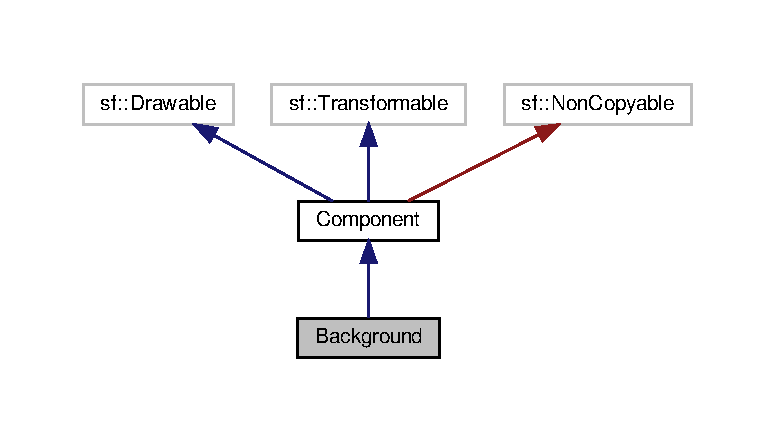
\includegraphics[width=350pt]{classBackground__inherit__graph}
\end{center}
\end{figure}


Collaboration diagram for Background\+:
\nopagebreak
\begin{figure}[H]
\begin{center}
\leavevmode
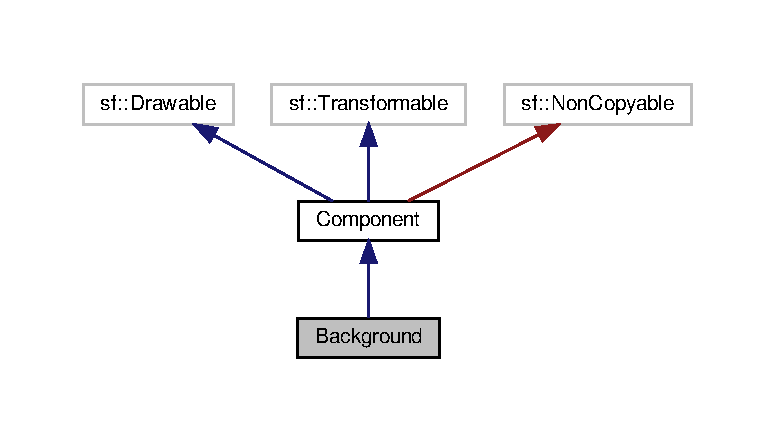
\includegraphics[width=350pt]{classBackground__coll__graph}
\end{center}
\end{figure}
\subsection*{Public Member Functions}
\begin{DoxyCompactItemize}
\item 
\hyperlink{classBackground_a7b34d3f65318880a36d9db9a5df60d85}{Background} (std\+::string path=\char`\"{}media/images/Galaxy2.\+png\char`\"{}, bool repeat=true, int opacity=255)
\begin{DoxyCompactList}\small\item\em Construct a new \hyperlink{classBackground}{Background} object. \end{DoxyCompactList}\item 
virtual bool \hyperlink{classBackground_acc764dce6ac4f8843bc9950dad313ee4}{is\+Selectable} () const
\begin{DoxyCompactList}\small\item\em get a confirmation bool \end{DoxyCompactList}\item 
\mbox{\Hypertarget{classBackground_a931546a41fa369074a955f806f7013ba}\label{classBackground_a931546a41fa369074a955f806f7013ba}} 
virtual bool {\bfseries update} (sf\+::\+Time dt)
\item 
\mbox{\Hypertarget{classBackground_ad8df5f7d22a79df18fb9b12058b09eb8}\label{classBackground_ad8df5f7d22a79df18fb9b12058b09eb8}} 
virtual void {\bfseries handle\+Event} (const sf\+::\+Event \&event)
\item 
void \hyperlink{classBackground_a015a2adae388abae75d6451273c61099}{set\+Size} (sf\+::\+Int\+Rect rect)
\begin{DoxyCompactList}\small\item\em Set the Size object. \end{DoxyCompactList}\item 
void \hyperlink{classBackground_a3c7b1c14ebc2ddad845e55eb2e214ce5}{set\+Path} (std\+::string path)
\begin{DoxyCompactList}\small\item\em Set the Path to where is the figure. \end{DoxyCompactList}\item 
void \hyperlink{classBackground_adee3f510209c8a2a53b4b2b2d27d27e5}{set\+Transparency} (float value)
\begin{DoxyCompactList}\small\item\em Set the background transparency level. \end{DoxyCompactList}\end{DoxyCompactItemize}


\subsection{Constructor \& Destructor Documentation}
\mbox{\Hypertarget{classBackground_a7b34d3f65318880a36d9db9a5df60d85}\label{classBackground_a7b34d3f65318880a36d9db9a5df60d85}} 
\index{Background@{Background}!Background@{Background}}
\index{Background@{Background}!Background@{Background}}
\subsubsection{\texorpdfstring{Background()}{Background()}}
{\footnotesize\ttfamily Background\+::\+Background (\begin{DoxyParamCaption}\item[{std\+::string}]{path = {\ttfamily \char`\"{}media/images/Galaxy2.png\char`\"{}},  }\item[{bool}]{repeat = {\ttfamily true},  }\item[{int}]{opacity = {\ttfamily 255} }\end{DoxyParamCaption})}



Construct a new \hyperlink{classBackground}{Background} object. 


\begin{DoxyParams}{Parameters}
{\em path} & background \\
\hline
{\em repeat} & if the image isn\textquotesingle{}t large enough \\
\hline
{\em opacity} & number from 0 to 255 for opacity; 128 for half transparent \\
\hline
\end{DoxyParams}


\subsection{Member Function Documentation}
\mbox{\Hypertarget{classBackground_acc764dce6ac4f8843bc9950dad313ee4}\label{classBackground_acc764dce6ac4f8843bc9950dad313ee4}} 
\index{Background@{Background}!is\+Selectable@{is\+Selectable}}
\index{is\+Selectable@{is\+Selectable}!Background@{Background}}
\subsubsection{\texorpdfstring{is\+Selectable()}{isSelectable()}}
{\footnotesize\ttfamily bool Background\+::is\+Selectable (\begin{DoxyParamCaption}{ }\end{DoxyParamCaption}) const\hspace{0.3cm}{\ttfamily [virtual]}}



get a confirmation bool 

\begin{DoxyReturn}{Returns}
the state 
\end{DoxyReturn}


Implements \hyperlink{classComponent_aede74a18a443413465216f383a046028}{Component}.

\mbox{\Hypertarget{classBackground_a3c7b1c14ebc2ddad845e55eb2e214ce5}\label{classBackground_a3c7b1c14ebc2ddad845e55eb2e214ce5}} 
\index{Background@{Background}!set\+Path@{set\+Path}}
\index{set\+Path@{set\+Path}!Background@{Background}}
\subsubsection{\texorpdfstring{set\+Path()}{setPath()}}
{\footnotesize\ttfamily void Background\+::set\+Path (\begin{DoxyParamCaption}\item[{std\+::string}]{path }\end{DoxyParamCaption})}



Set the Path to where is the figure. 


\begin{DoxyParams}{Parameters}
{\em path} & \\
\hline
\end{DoxyParams}
\mbox{\Hypertarget{classBackground_a015a2adae388abae75d6451273c61099}\label{classBackground_a015a2adae388abae75d6451273c61099}} 
\index{Background@{Background}!set\+Size@{set\+Size}}
\index{set\+Size@{set\+Size}!Background@{Background}}
\subsubsection{\texorpdfstring{set\+Size()}{setSize()}}
{\footnotesize\ttfamily void Background\+::set\+Size (\begin{DoxyParamCaption}\item[{sf\+::\+Int\+Rect}]{rect }\end{DoxyParamCaption})}



Set the Size object. 


\begin{DoxyParams}{Parameters}
{\em rect} & sf\+::\+Int\+Rect object \\
\hline
\end{DoxyParams}
\mbox{\Hypertarget{classBackground_adee3f510209c8a2a53b4b2b2d27d27e5}\label{classBackground_adee3f510209c8a2a53b4b2b2d27d27e5}} 
\index{Background@{Background}!set\+Transparency@{set\+Transparency}}
\index{set\+Transparency@{set\+Transparency}!Background@{Background}}
\subsubsection{\texorpdfstring{set\+Transparency()}{setTransparency()}}
{\footnotesize\ttfamily void Background\+::set\+Transparency (\begin{DoxyParamCaption}\item[{float}]{value }\end{DoxyParamCaption})}



Set the background transparency level. 


\begin{DoxyParams}{Parameters}
{\em value} & between 0(total invisble) and 255(normal) \\
\hline
\end{DoxyParams}


The documentation for this class was generated from the following files\+:\begin{DoxyCompactItemize}
\item 
sources/utils/\+Components/Background.\+hpp\item 
sources/utils/\+Components/Background.\+cpp\end{DoxyCompactItemize}

\hypertarget{classButton}{}\section{Button Class Reference}
\label{classButton}\index{Button@{Button}}


abstraction of a button component to implement in the view  




{\ttfamily \#include $<$Button.\+hpp$>$}



Inheritance diagram for Button\+:
\nopagebreak
\begin{figure}[H]
\begin{center}
\leavevmode
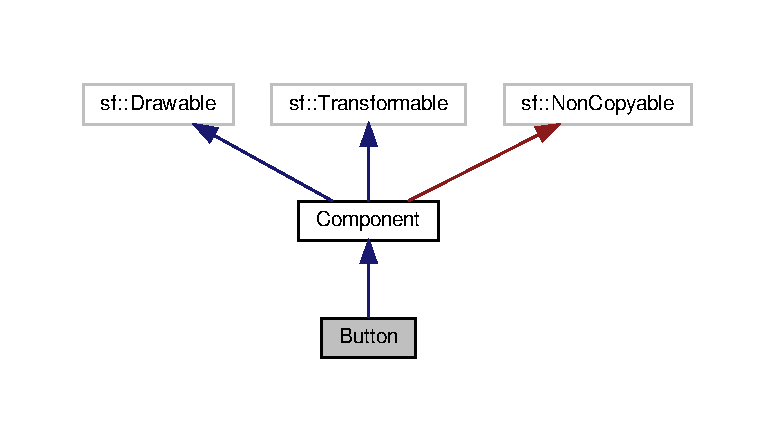
\includegraphics[width=350pt]{classButton__inherit__graph}
\end{center}
\end{figure}


Collaboration diagram for Button\+:
\nopagebreak
\begin{figure}[H]
\begin{center}
\leavevmode
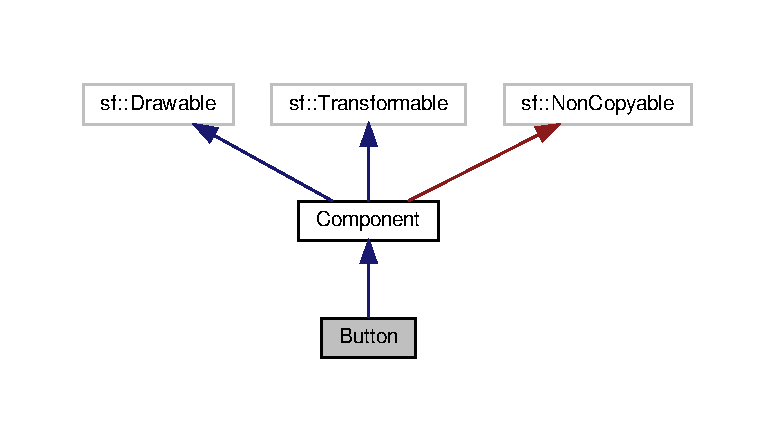
\includegraphics[width=350pt]{classButton__coll__graph}
\end{center}
\end{figure}
\subsection*{Public Types}
\begin{DoxyCompactItemize}
\item 
\mbox{\Hypertarget{classButton_a9e04a84d89368e9a5b1205bbcdd1a9b0}\label{classButton_a9e04a84d89368e9a5b1205bbcdd1a9b0}} 
typedef std\+::function$<$ void()$>$ {\bfseries Callback}
\end{DoxyCompactItemize}
\subsection*{Public Member Functions}
\begin{DoxyCompactItemize}
\item 
\hyperlink{classButton_a421ba03df1f2038625a179d72ade06a8}{Button} (const std\+::string \&text, const std\+::string \&path, bool active, float size, bool pred=false)
\begin{DoxyCompactList}\small\item\em Construct a new \hyperlink{classButton}{Button} object. \end{DoxyCompactList}\item 
void \hyperlink{classButton_ac6a233c876164a52d54ef7f1b3fb78d1}{set\+Text} (const std\+::string \&text)
\begin{DoxyCompactList}\small\item\em Set the Text object. \end{DoxyCompactList}\item 
void \hyperlink{classButton_a694455fc4d23bf1dd91836f9692933ad}{set\+Callback} (Callback callback)
\begin{DoxyCompactList}\small\item\em Set the Callback function in which the button will then activate. \end{DoxyCompactList}\item 
virtual bool \hyperlink{classButton_a6f51f01b72f9c3319e96263dc59a677f}{is\+Selectable} () const
\begin{DoxyCompactList}\small\item\em Return state of selecting. \end{DoxyCompactList}\item 
\mbox{\Hypertarget{classButton_a0d567e275b73139fe0300f395f657656}\label{classButton_a0d567e275b73139fe0300f395f657656}} 
virtual void \hyperlink{classButton_a0d567e275b73139fe0300f395f657656}{select} ()
\begin{DoxyCompactList}\small\item\em changes the button layout and plays selection music \end{DoxyCompactList}\item 
\mbox{\Hypertarget{classButton_a565331dbe481e0f55e26a4a1f36ee40e}\label{classButton_a565331dbe481e0f55e26a4a1f36ee40e}} 
virtual void \hyperlink{classButton_a565331dbe481e0f55e26a4a1f36ee40e}{deselect} ()
\begin{DoxyCompactList}\small\item\em deselect the button \end{DoxyCompactList}\item 
\mbox{\Hypertarget{classButton_a78bc21a32f143adf0de1204e6f230629}\label{classButton_a78bc21a32f143adf0de1204e6f230629}} 
void \hyperlink{classButton_a78bc21a32f143adf0de1204e6f230629}{toggle} ()
\begin{DoxyCompactList}\small\item\em Alternate button status and play switching music. \end{DoxyCompactList}\item 
virtual void \hyperlink{classButton_a2fe7d7228fb882c5c992ed07341d45be}{activate} ()
\begin{DoxyCompactList}\small\item\em Take action if this going to be activate unimplemented. \end{DoxyCompactList}\item 
virtual void \hyperlink{classButton_a57efb09b51a4846a25e7f61abee78cd6}{deactivate} ()
\begin{DoxyCompactList}\small\item\em Take action if this going to be activate unimplemented. \end{DoxyCompactList}\item 
\mbox{\Hypertarget{classButton_ac0c49438494d666916359871ce76f541}\label{classButton_ac0c49438494d666916359871ce76f541}} 
virtual bool {\bfseries update} (sf\+::\+Time dt)
\item 
\mbox{\Hypertarget{classButton_a1c97f0b778e1b6cb45818b3573b71487}\label{classButton_a1c97f0b778e1b6cb45818b3573b71487}} 
virtual void {\bfseries handle\+Event} (const sf\+::\+Event \&event)
\end{DoxyCompactItemize}


\subsection{Detailed Description}
abstraction of a button component to implement in the view 

\subsection{Constructor \& Destructor Documentation}
\mbox{\Hypertarget{classButton_a421ba03df1f2038625a179d72ade06a8}\label{classButton_a421ba03df1f2038625a179d72ade06a8}} 
\index{Button@{Button}!Button@{Button}}
\index{Button@{Button}!Button@{Button}}
\subsubsection{\texorpdfstring{Button()}{Button()}}
{\footnotesize\ttfamily Button\+::\+Button (\begin{DoxyParamCaption}\item[{const std\+::string \&}]{text,  }\item[{const std\+::string \&}]{path,  }\item[{bool}]{active,  }\item[{float}]{size,  }\item[{bool}]{pred = {\ttfamily false} }\end{DoxyParamCaption})}



Construct a new \hyperlink{classButton}{Button} object. 


\begin{DoxyParams}{Parameters}
{\em text} & button text \\
\hline
{\em path} & font path \\
\hline
{\em active} & visible or not \\
\hline
{\em size} & \\
\hline
{\em pred} & selected or not \\
\hline
\end{DoxyParams}


\subsection{Member Function Documentation}
\mbox{\Hypertarget{classButton_a2fe7d7228fb882c5c992ed07341d45be}\label{classButton_a2fe7d7228fb882c5c992ed07341d45be}} 
\index{Button@{Button}!activate@{activate}}
\index{activate@{activate}!Button@{Button}}
\subsubsection{\texorpdfstring{activate()}{activate()}}
{\footnotesize\ttfamily void Button\+::activate (\begin{DoxyParamCaption}{ }\end{DoxyParamCaption})\hspace{0.3cm}{\ttfamily [virtual]}}



Take action if this going to be activate unimplemented. 

T\+O\+DO\+: In the future place here what to do when selected and activated or deactivated

Reimplemented from \hyperlink{classComponent_aaab29ea159109b4d0f63e9c519be6139}{Component}.

\mbox{\Hypertarget{classButton_a57efb09b51a4846a25e7f61abee78cd6}\label{classButton_a57efb09b51a4846a25e7f61abee78cd6}} 
\index{Button@{Button}!deactivate@{deactivate}}
\index{deactivate@{deactivate}!Button@{Button}}
\subsubsection{\texorpdfstring{deactivate()}{deactivate()}}
{\footnotesize\ttfamily void Button\+::deactivate (\begin{DoxyParamCaption}{ }\end{DoxyParamCaption})\hspace{0.3cm}{\ttfamily [virtual]}}



Take action if this going to be activate unimplemented. 

T\+O\+DO\+: In the future place here what to do when selected and activated or deactivated

Reimplemented from \hyperlink{classComponent_aa4d1e5e0656ed03f7ff469db25f65053}{Component}.

\mbox{\Hypertarget{classButton_a6f51f01b72f9c3319e96263dc59a677f}\label{classButton_a6f51f01b72f9c3319e96263dc59a677f}} 
\index{Button@{Button}!is\+Selectable@{is\+Selectable}}
\index{is\+Selectable@{is\+Selectable}!Button@{Button}}
\subsubsection{\texorpdfstring{is\+Selectable()}{isSelectable()}}
{\footnotesize\ttfamily bool Button\+::is\+Selectable (\begin{DoxyParamCaption}{ }\end{DoxyParamCaption}) const\hspace{0.3cm}{\ttfamily [virtual]}}



Return state of selecting. 

\begin{DoxyReturn}{Returns}
true 

false 
\end{DoxyReturn}


Implements \hyperlink{classComponent_aede74a18a443413465216f383a046028}{Component}.

\mbox{\Hypertarget{classButton_a694455fc4d23bf1dd91836f9692933ad}\label{classButton_a694455fc4d23bf1dd91836f9692933ad}} 
\index{Button@{Button}!set\+Callback@{set\+Callback}}
\index{set\+Callback@{set\+Callback}!Button@{Button}}
\subsubsection{\texorpdfstring{set\+Callback()}{setCallback()}}
{\footnotesize\ttfamily void Button\+::set\+Callback (\begin{DoxyParamCaption}\item[{Callback}]{callback }\end{DoxyParamCaption})}



Set the Callback function in which the button will then activate. 


\begin{DoxyParams}{Parameters}
{\em callback} & \\
\hline
\end{DoxyParams}
\mbox{\Hypertarget{classButton_ac6a233c876164a52d54ef7f1b3fb78d1}\label{classButton_ac6a233c876164a52d54ef7f1b3fb78d1}} 
\index{Button@{Button}!set\+Text@{set\+Text}}
\index{set\+Text@{set\+Text}!Button@{Button}}
\subsubsection{\texorpdfstring{set\+Text()}{setText()}}
{\footnotesize\ttfamily void Button\+::set\+Text (\begin{DoxyParamCaption}\item[{const std\+::string \&}]{text }\end{DoxyParamCaption})}



Set the Text object. 


\begin{DoxyParams}{Parameters}
{\em text} & \\
\hline
\end{DoxyParams}


The documentation for this class was generated from the following files\+:\begin{DoxyCompactItemize}
\item 
sources/utils/\+Components/Button.\+hpp\item 
sources/utils/\+Components/Button.\+cpp\end{DoxyCompactItemize}

\hypertarget{classClient}{}\section{Client Class Reference}
\label{classClient}\index{Client@{Client}}
\subsection*{Public Member Functions}
\begin{DoxyCompactItemize}
\item 
\mbox{\Hypertarget{classClient_a9dacbc3677315e923e8c50e50db6725e}\label{classClient_a9dacbc3677315e923e8c50e50db6725e}} 
R\+E\+S\+P\+O\+N\+S\+E\+\_\+\+S\+T\+A\+T\+US {\bfseries search\+Conection} ()
\item 
\mbox{\Hypertarget{classClient_a0ad050c35231e71ded2ffdd83a2a1ea7}\label{classClient_a0ad050c35231e71ded2ffdd83a2a1ea7}} 
R\+E\+S\+P\+O\+N\+S\+E\+\_\+\+S\+T\+A\+T\+US {\bfseries listen\+Conection} ()
\item 
\mbox{\Hypertarget{classClient_aa675dea94e1a5b19e37bd19d35a99620}\label{classClient_aa675dea94e1a5b19e37bd19d35a99620}} 
sf\+::\+Ip\+Address {\bfseries get\+Receiver} ()
\item 
\mbox{\Hypertarget{classClient_a5ea44065fefaa5d96709fb59082a0fcd}\label{classClient_a5ea44065fefaa5d96709fb59082a0fcd}} 
void {\bfseries set\+Receiver} (sf\+::\+Ip\+Address ia)
\item 
\mbox{\Hypertarget{classClient_a65d2e1dcab3412f1df6b30f97265f909}\label{classClient_a65d2e1dcab3412f1df6b30f97265f909}} 
void {\bfseries establish\+Port} (bool create)
\item 
\mbox{\Hypertarget{classClient_ace8e511813b9b461570bc0bf5b9a2307}\label{classClient_ace8e511813b9b461570bc0bf5b9a2307}} 
void {\bfseries recv\+Data} (std\+::vector$<$ int $>$ \&v)
\item 
\mbox{\Hypertarget{classClient_a52dd5c67c4a0f52f62706eb2a96bfa0d}\label{classClient_a52dd5c67c4a0f52f62706eb2a96bfa0d}} 
void {\bfseries send\+Data} (std\+::vector$<$ int $>$ v)
\end{DoxyCompactItemize}


The documentation for this class was generated from the following files\+:\begin{DoxyCompactItemize}
\item 
sources/network/Client.\+hpp\item 
sources/network/Client.\+cpp\end{DoxyCompactItemize}

\hypertarget{classComponent}{}\section{Component Class Reference}
\label{classComponent}\index{Component@{Component}}


Mother class for the components created, which compiles S\+F\+ML functions.  




{\ttfamily \#include $<$Component.\+hpp$>$}



Inheritance diagram for Component\+:
\nopagebreak
\begin{figure}[H]
\begin{center}
\leavevmode
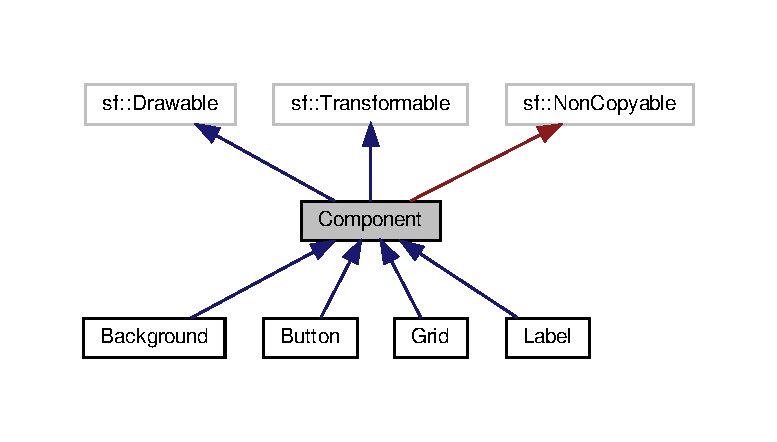
\includegraphics[width=350pt]{classComponent__inherit__graph}
\end{center}
\end{figure}


Collaboration diagram for Component\+:
\nopagebreak
\begin{figure}[H]
\begin{center}
\leavevmode
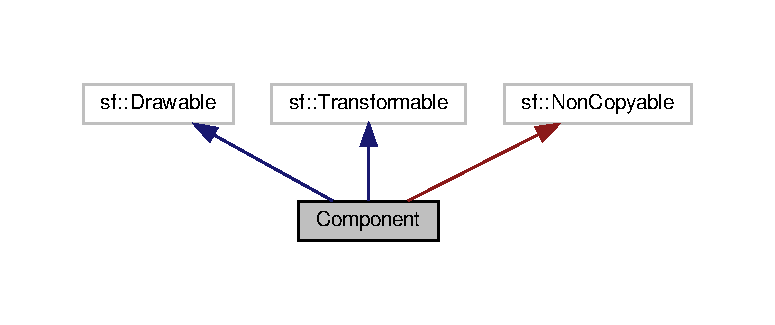
\includegraphics[width=350pt]{classComponent__coll__graph}
\end{center}
\end{figure}
\subsection*{Public Member Functions}
\begin{DoxyCompactItemize}
\item 
\mbox{\Hypertarget{classComponent_a8775db6d1a2c1afc2e77cd3c8f39da6f}\label{classComponent_a8775db6d1a2c1afc2e77cd3c8f39da6f}} 
\hyperlink{classComponent_a8775db6d1a2c1afc2e77cd3c8f39da6f}{Component} ()
\begin{DoxyCompactList}\small\item\em Construct a new \hyperlink{classComponent}{Component} object. \end{DoxyCompactList}\item 
virtual bool \hyperlink{classComponent_aede74a18a443413465216f383a046028}{is\+Selectable} () const =0
\begin{DoxyCompactList}\small\item\em get a confirmation bool \end{DoxyCompactList}\item 
bool \hyperlink{classComponent_a4c480061afaabc44339ca63916711294}{is\+Selected} () const
\begin{DoxyCompactList}\small\item\em get a confirmation bool \end{DoxyCompactList}\item 
\mbox{\Hypertarget{classComponent_ad92e03b1674737ed690eb72a0ad507f2}\label{classComponent_ad92e03b1674737ed690eb72a0ad507f2}} 
virtual void \hyperlink{classComponent_ad92e03b1674737ed690eb72a0ad507f2}{select} ()
\begin{DoxyCompactList}\small\item\em select the component \end{DoxyCompactList}\item 
\mbox{\Hypertarget{classComponent_abe3bf558cf657c6da9ac30929fce5ed2}\label{classComponent_abe3bf558cf657c6da9ac30929fce5ed2}} 
virtual void \hyperlink{classComponent_abe3bf558cf657c6da9ac30929fce5ed2}{deselect} ()
\begin{DoxyCompactList}\small\item\em deselect the component \end{DoxyCompactList}\item 
virtual bool \hyperlink{classComponent_ad9a1fae6416df7f295c603483f15ce4a}{is\+Active} () const
\begin{DoxyCompactList}\small\item\em get a confirmation bool \end{DoxyCompactList}\item 
\mbox{\Hypertarget{classComponent_aaab29ea159109b4d0f63e9c519be6139}\label{classComponent_aaab29ea159109b4d0f63e9c519be6139}} 
virtual void \hyperlink{classComponent_aaab29ea159109b4d0f63e9c519be6139}{activate} ()
\begin{DoxyCompactList}\small\item\em active the component \end{DoxyCompactList}\item 
\mbox{\Hypertarget{classComponent_aa4d1e5e0656ed03f7ff469db25f65053}\label{classComponent_aa4d1e5e0656ed03f7ff469db25f65053}} 
virtual void \hyperlink{classComponent_aa4d1e5e0656ed03f7ff469db25f65053}{deactivate} ()
\begin{DoxyCompactList}\small\item\em deactive the component \end{DoxyCompactList}\item 
\mbox{\Hypertarget{classComponent_a090d3bc2747d4538799a1f92599ec899}\label{classComponent_a090d3bc2747d4538799a1f92599ec899}} 
virtual bool {\bfseries update} (sf\+::\+Time dt)=0
\item 
\mbox{\Hypertarget{classComponent_a75ed67b03624574c7c45a26eda11a46e}\label{classComponent_a75ed67b03624574c7c45a26eda11a46e}} 
virtual void {\bfseries handle\+Event} (const sf\+::\+Event \&event)=0
\end{DoxyCompactItemize}


\subsection{Detailed Description}
Mother class for the components created, which compiles S\+F\+ML functions. 

\subsection{Member Function Documentation}
\mbox{\Hypertarget{classComponent_ad9a1fae6416df7f295c603483f15ce4a}\label{classComponent_ad9a1fae6416df7f295c603483f15ce4a}} 
\index{Component@{Component}!is\+Active@{is\+Active}}
\index{is\+Active@{is\+Active}!Component@{Component}}
\subsubsection{\texorpdfstring{is\+Active()}{isActive()}}
{\footnotesize\ttfamily bool Component\+::is\+Active (\begin{DoxyParamCaption}{ }\end{DoxyParamCaption}) const\hspace{0.3cm}{\ttfamily [virtual]}}



get a confirmation bool 

\begin{DoxyReturn}{Returns}
the state 
\end{DoxyReturn}
\mbox{\Hypertarget{classComponent_aede74a18a443413465216f383a046028}\label{classComponent_aede74a18a443413465216f383a046028}} 
\index{Component@{Component}!is\+Selectable@{is\+Selectable}}
\index{is\+Selectable@{is\+Selectable}!Component@{Component}}
\subsubsection{\texorpdfstring{is\+Selectable()}{isSelectable()}}
{\footnotesize\ttfamily virtual bool Component\+::is\+Selectable (\begin{DoxyParamCaption}{ }\end{DoxyParamCaption}) const\hspace{0.3cm}{\ttfamily [pure virtual]}}



get a confirmation bool 

\begin{DoxyReturn}{Returns}
the state 
\end{DoxyReturn}


Implemented in \hyperlink{classButton_a6f51f01b72f9c3319e96263dc59a677f}{Button}, \hyperlink{classGrid_a4ef4763b55dc2696af8a71fdeabe999a}{Grid}, \hyperlink{classLabel_ac27e6e31942be4612d282af282b65051}{Label}, and \hyperlink{classBackground_acc764dce6ac4f8843bc9950dad313ee4}{Background}.

\mbox{\Hypertarget{classComponent_a4c480061afaabc44339ca63916711294}\label{classComponent_a4c480061afaabc44339ca63916711294}} 
\index{Component@{Component}!is\+Selected@{is\+Selected}}
\index{is\+Selected@{is\+Selected}!Component@{Component}}
\subsubsection{\texorpdfstring{is\+Selected()}{isSelected()}}
{\footnotesize\ttfamily bool Component\+::is\+Selected (\begin{DoxyParamCaption}{ }\end{DoxyParamCaption}) const}



get a confirmation bool 

\begin{DoxyReturn}{Returns}
the state 
\end{DoxyReturn}


The documentation for this class was generated from the following files\+:\begin{DoxyCompactItemize}
\item 
sources/utils/\+Components/Component.\+hpp\item 
sources/utils/\+Components/Component.\+cpp\end{DoxyCompactItemize}

\hypertarget{structState_1_1Context}{}\section{State\+:\+:Context Struct Reference}
\label{structState_1_1Context}\index{State\+::\+Context@{State\+::\+Context}}


structure that references the current context screen  




{\ttfamily \#include $<$State.\+hpp$>$}



Collaboration diagram for State\+:\+:Context\+:
\nopagebreak
\begin{figure}[H]
\begin{center}
\leavevmode
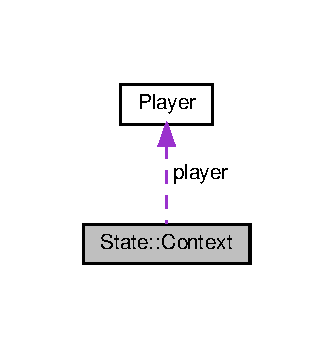
\includegraphics[width=160pt]{structState_1_1Context__coll__graph}
\end{center}
\end{figure}
\subsection*{Public Member Functions}
\begin{DoxyCompactItemize}
\item 
\mbox{\Hypertarget{structState_1_1Context_a8016ecde0d28a4df5ea03a0609e5c2d1}\label{structState_1_1Context_a8016ecde0d28a4df5ea03a0609e5c2d1}} 
{\bfseries Context} (sf\+::\+Render\+Window \&window, \hyperlink{classPlayer}{Player} \&player)
\end{DoxyCompactItemize}
\subsection*{Public Attributes}
\begin{DoxyCompactItemize}
\item 
\mbox{\Hypertarget{structState_1_1Context_a30775e70e841c761a4e3cb7f0e195128}\label{structState_1_1Context_a30775e70e841c761a4e3cb7f0e195128}} 
sf\+::\+Render\+Window $\ast$ {\bfseries window}
\item 
\mbox{\Hypertarget{structState_1_1Context_a1c98434687748acdebf78fd80a4767ad}\label{structState_1_1Context_a1c98434687748acdebf78fd80a4767ad}} 
\hyperlink{classPlayer}{Player} $\ast$ {\bfseries player}
\end{DoxyCompactItemize}


\subsection{Detailed Description}
structure that references the current context screen 

The documentation for this struct was generated from the following files\+:\begin{DoxyCompactItemize}
\item 
sources/utils/\+States/State.\+hpp\item 
sources/utils/\+States/State.\+cpp\end{DoxyCompactItemize}

\hypertarget{classGameScene}{}\section{Game\+Scene Class Reference}
\label{classGameScene}\index{Game\+Scene@{Game\+Scene}}


responsible for sampling the main screen of the singleplayer game  




{\ttfamily \#include $<$Game\+Scene.\+hpp$>$}



Inheritance diagram for Game\+Scene\+:
\nopagebreak
\begin{figure}[H]
\begin{center}
\leavevmode
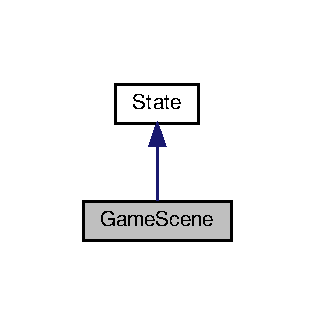
\includegraphics[width=151pt]{classGameScene__inherit__graph}
\end{center}
\end{figure}


Collaboration diagram for Game\+Scene\+:
\nopagebreak
\begin{figure}[H]
\begin{center}
\leavevmode
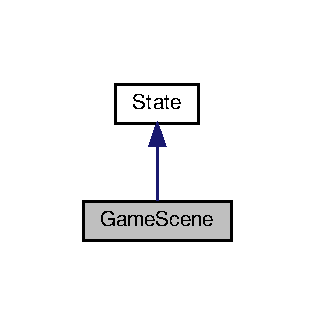
\includegraphics[width=151pt]{classGameScene__coll__graph}
\end{center}
\end{figure}
\subsection*{Public Member Functions}
\begin{DoxyCompactItemize}
\item 
\hyperlink{classGameScene_abc5dab6de1f960181d01c4991c15a3e8}{Game\+Scene} (\hyperlink{classStateManager}{State\+Manager} \&stack, \hyperlink{structState_1_1Context}{Context} context)
\begin{DoxyCompactList}\small\item\em Construct a new Multiplayer Scene object, standard builder. \end{DoxyCompactList}\item 
\mbox{\Hypertarget{classGameScene_ae9eb60cbb8fa55eeb07b951e3d83f426}\label{classGameScene_ae9eb60cbb8fa55eeb07b951e3d83f426}} 
virtual void \hyperlink{classGameScene_ae9eb60cbb8fa55eeb07b951e3d83f426}{draw} ()
\begin{DoxyCompactList}\small\item\em overwriting the function drawing by adding new elements responsible for sampling new elements added to this view \end{DoxyCompactList}\item 
virtual bool \hyperlink{classGameScene_ac47e1a8082955a6c7af92cf7dbdd9347}{update} (sf\+::\+Time dt)
\begin{DoxyCompactList}\small\item\em overwriting the function update by adding new elements responsible for sampling new elements added to this view \end{DoxyCompactList}\item 
virtual bool \hyperlink{classGameScene_aa494372b1f451f3c3a268558fddb30f2}{handle\+Event} (const sf\+::\+Event \&event)
\begin{DoxyCompactList}\small\item\em Adds new features to the function responsible for handling the events, adding a specific function for each key depending on the view. \end{DoxyCompactList}\item 
\mbox{\Hypertarget{classGameScene_aa3729415c97d2bcf67add017213d0f27}\label{classGameScene_aa3729415c97d2bcf67add017213d0f27}} 
std\+::string {\bfseries get\+Human\+Time} (sf\+::\+Time dt) const
\end{DoxyCompactItemize}
\subsection*{Additional Inherited Members}


\subsection{Detailed Description}
responsible for sampling the main screen of the singleplayer game 

\subsection{Constructor \& Destructor Documentation}
\mbox{\Hypertarget{classGameScene_abc5dab6de1f960181d01c4991c15a3e8}\label{classGameScene_abc5dab6de1f960181d01c4991c15a3e8}} 
\index{Game\+Scene@{Game\+Scene}!Game\+Scene@{Game\+Scene}}
\index{Game\+Scene@{Game\+Scene}!Game\+Scene@{Game\+Scene}}
\subsubsection{\texorpdfstring{Game\+Scene()}{GameScene()}}
{\footnotesize\ttfamily Game\+Scene\+::\+Game\+Scene (\begin{DoxyParamCaption}\item[{\hyperlink{classStateManager}{State\+Manager} \&}]{stack,  }\item[{\hyperlink{structState_1_1Context}{Context}}]{context }\end{DoxyParamCaption})}



Construct a new Multiplayer Scene object, standard builder. 


\begin{DoxyParams}{Parameters}
{\em stack} & stack responsible for managing the views \\
\hline
{\em context} & relates all current context \\
\hline
\end{DoxyParams}
T\+O\+DO\+: Optimize the exchange between single and multiplayer Optimize the change of variables between singleplayer and multiplayer

\subsection{Member Function Documentation}
\mbox{\Hypertarget{classGameScene_aa494372b1f451f3c3a268558fddb30f2}\label{classGameScene_aa494372b1f451f3c3a268558fddb30f2}} 
\index{Game\+Scene@{Game\+Scene}!handle\+Event@{handle\+Event}}
\index{handle\+Event@{handle\+Event}!Game\+Scene@{Game\+Scene}}
\subsubsection{\texorpdfstring{handle\+Event()}{handleEvent()}}
{\footnotesize\ttfamily bool Game\+Scene\+::handle\+Event (\begin{DoxyParamCaption}\item[{const sf\+::\+Event \&}]{event }\end{DoxyParamCaption})\hspace{0.3cm}{\ttfamily [virtual]}}



Adds new features to the function responsible for handling the events, adding a specific function for each key depending on the view. 


\begin{DoxyParams}{Parameters}
{\em event} & getted action \\
\hline
\end{DoxyParams}
\begin{DoxyReturn}{Returns}
true 

false if have a problem 
\end{DoxyReturn}


Implements \hyperlink{classState_a19965f83460b248c42952aac8d001206}{State}.

\mbox{\Hypertarget{classGameScene_ac47e1a8082955a6c7af92cf7dbdd9347}\label{classGameScene_ac47e1a8082955a6c7af92cf7dbdd9347}} 
\index{Game\+Scene@{Game\+Scene}!update@{update}}
\index{update@{update}!Game\+Scene@{Game\+Scene}}
\subsubsection{\texorpdfstring{update()}{update()}}
{\footnotesize\ttfamily bool Game\+Scene\+::update (\begin{DoxyParamCaption}\item[{sf\+::\+Time}]{dt }\end{DoxyParamCaption})\hspace{0.3cm}{\ttfamily [virtual]}}



overwriting the function update by adding new elements responsible for sampling new elements added to this view 


\begin{DoxyParams}{Parameters}
{\em dt} & Fraction of time \\
\hline
\end{DoxyParams}
\begin{DoxyReturn}{Returns}
true 

false if have a problem 
\end{DoxyReturn}


Implements \hyperlink{classState_acd5926bc7a373edff9e57f3ffe94ca13}{State}.



The documentation for this class was generated from the following files\+:\begin{DoxyCompactItemize}
\item 
sources/views/Game\+Scene.\+hpp\item 
sources/views/Game\+Scene.\+cpp\end{DoxyCompactItemize}

\hypertarget{classGrid}{}\section{Grid Class Reference}
\label{classGrid}\index{Grid@{Grid}}


build the meshes responsible for making the tetris table  




{\ttfamily \#include $<$Grid.\+hpp$>$}



Inheritance diagram for Grid\+:
\nopagebreak
\begin{figure}[H]
\begin{center}
\leavevmode
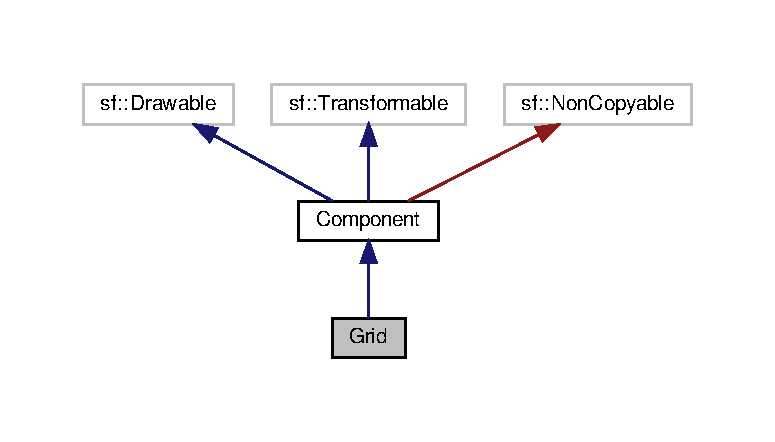
\includegraphics[width=350pt]{classGrid__inherit__graph}
\end{center}
\end{figure}


Collaboration diagram for Grid\+:
\nopagebreak
\begin{figure}[H]
\begin{center}
\leavevmode
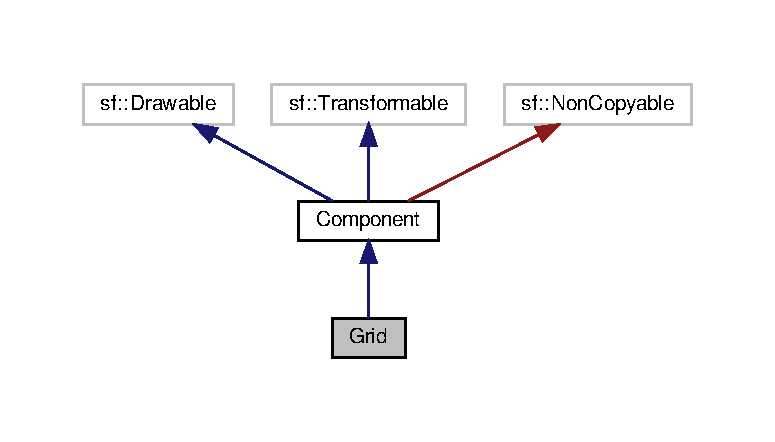
\includegraphics[width=350pt]{classGrid__coll__graph}
\end{center}
\end{figure}
\subsection*{Public Member Functions}
\begin{DoxyCompactItemize}
\item 
\hyperlink{classGrid_ae4e9e4e01ed8d1ffe5f4bf560680362e}{Grid} (int m\+Height, int m\+Width, float m\+Pixel=30)
\begin{DoxyCompactList}\small\item\em Construct a new \hyperlink{classGrid}{Grid} object. \end{DoxyCompactList}\item 
virtual bool \hyperlink{classGrid_a4ef4763b55dc2696af8a71fdeabe999a}{is\+Selectable} () const
\begin{DoxyCompactList}\small\item\em get a confirmation bool \end{DoxyCompactList}\item 
\mbox{\Hypertarget{classGrid_acaae18fea153b8ad2973597b7db449f9}\label{classGrid_acaae18fea153b8ad2973597b7db449f9}} 
void {\bfseries set\+Text} (const std\+::string \&text)
\item 
\mbox{\Hypertarget{classGrid_aa933917cfed17cc246121c16ee2621ed}\label{classGrid_aa933917cfed17cc246121c16ee2621ed}} 
virtual bool {\bfseries update} (sf\+::\+Time dt)
\item 
\mbox{\Hypertarget{classGrid_a2e0f15ff4079c91bfb40e519268a09b9}\label{classGrid_a2e0f15ff4079c91bfb40e519268a09b9}} 
virtual void {\bfseries handle\+Event} (const sf\+::\+Event \&event)
\item 
void \hyperlink{classGrid_a7a93d93a3acaac29bc8fa81ecf30f877}{set\+Colors} (const std\+::vector$<$ int $>$ \&v)
\begin{DoxyCompactList}\small\item\em Set the Colors object. \end{DoxyCompactList}\item 
\mbox{\Hypertarget{classGrid_a4a7063b92ed09312e51c4a7fa0c2a0f0}\label{classGrid_a4a7063b92ed09312e51c4a7fa0c2a0f0}} 
void {\bfseries restart} ()
\end{DoxyCompactItemize}


\subsection{Detailed Description}
build the meshes responsible for making the tetris table 

\subsection{Constructor \& Destructor Documentation}
\mbox{\Hypertarget{classGrid_ae4e9e4e01ed8d1ffe5f4bf560680362e}\label{classGrid_ae4e9e4e01ed8d1ffe5f4bf560680362e}} 
\index{Grid@{Grid}!Grid@{Grid}}
\index{Grid@{Grid}!Grid@{Grid}}
\subsubsection{\texorpdfstring{Grid()}{Grid()}}
{\footnotesize\ttfamily Grid\+::\+Grid (\begin{DoxyParamCaption}\item[{int}]{m\+Height,  }\item[{int}]{m\+Width,  }\item[{float}]{m\+Pixel = {\ttfamily 30} }\end{DoxyParamCaption})}



Construct a new \hyperlink{classGrid}{Grid} object. 


\begin{DoxyParams}{Parameters}
{\em m\+Height} & \\
\hline
{\em m\+Width} & \\
\hline
{\em m\+Pixel} & \\
\hline
\end{DoxyParams}


\subsection{Member Function Documentation}
\mbox{\Hypertarget{classGrid_a4ef4763b55dc2696af8a71fdeabe999a}\label{classGrid_a4ef4763b55dc2696af8a71fdeabe999a}} 
\index{Grid@{Grid}!is\+Selectable@{is\+Selectable}}
\index{is\+Selectable@{is\+Selectable}!Grid@{Grid}}
\subsubsection{\texorpdfstring{is\+Selectable()}{isSelectable()}}
{\footnotesize\ttfamily bool Grid\+::is\+Selectable (\begin{DoxyParamCaption}{ }\end{DoxyParamCaption}) const\hspace{0.3cm}{\ttfamily [virtual]}}



get a confirmation bool 

\begin{DoxyReturn}{Returns}
the state 
\end{DoxyReturn}


Implements \hyperlink{classComponent_aede74a18a443413465216f383a046028}{Component}.

\mbox{\Hypertarget{classGrid_a7a93d93a3acaac29bc8fa81ecf30f877}\label{classGrid_a7a93d93a3acaac29bc8fa81ecf30f877}} 
\index{Grid@{Grid}!set\+Colors@{set\+Colors}}
\index{set\+Colors@{set\+Colors}!Grid@{Grid}}
\subsubsection{\texorpdfstring{set\+Colors()}{setColors()}}
{\footnotesize\ttfamily void Grid\+::set\+Colors (\begin{DoxyParamCaption}\item[{const std\+::vector$<$ int $>$ \&}]{v }\end{DoxyParamCaption})}



Set the Colors object. 


\begin{DoxyParams}{Parameters}
{\em v} & color value in enum \\
\hline
\end{DoxyParams}


The documentation for this class was generated from the following files\+:\begin{DoxyCompactItemize}
\item 
sources/utils/\+Components/Grid.\+hpp\item 
sources/utils/\+Components/Grid.\+cpp\end{DoxyCompactItemize}

\hypertarget{classHelpScene}{}\section{Help\+Scene Class Reference}
\label{classHelpScene}\index{Help\+Scene@{Help\+Scene}}


responsible for viewing the help page of the game  




{\ttfamily \#include $<$Help\+Scene.\+hpp$>$}



Inheritance diagram for Help\+Scene\+:
\nopagebreak
\begin{figure}[H]
\begin{center}
\leavevmode
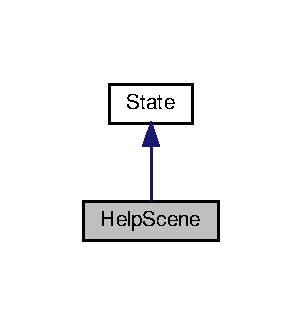
\includegraphics[width=145pt]{classHelpScene__inherit__graph}
\end{center}
\end{figure}


Collaboration diagram for Help\+Scene\+:
\nopagebreak
\begin{figure}[H]
\begin{center}
\leavevmode
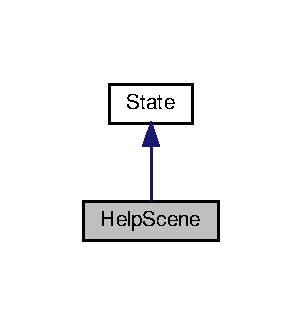
\includegraphics[width=145pt]{classHelpScene__coll__graph}
\end{center}
\end{figure}
\subsection*{Public Member Functions}
\begin{DoxyCompactItemize}
\item 
\hyperlink{classHelpScene_a97b066a6f6341021d0bc07a548ec3f6c}{Help\+Scene} (\hyperlink{classStateManager}{State\+Manager} \&stack, \hyperlink{structState_1_1Context}{Context} context)
\begin{DoxyCompactList}\small\item\em Construct a new Menu Scene object, standard builder. \end{DoxyCompactList}\item 
\mbox{\Hypertarget{classHelpScene_a1c343c3ede7bb3d3a6cb4f0d0eba3e53}\label{classHelpScene_a1c343c3ede7bb3d3a6cb4f0d0eba3e53}} 
virtual void \hyperlink{classHelpScene_a1c343c3ede7bb3d3a6cb4f0d0eba3e53}{draw} ()
\begin{DoxyCompactList}\small\item\em overwriting the function drawing by adding new elements responsible for sampling new elements added to this view \end{DoxyCompactList}\item 
virtual bool \hyperlink{classHelpScene_a2eb8b8e49f206b65291a8972f3c596c0}{update} (sf\+::\+Time dt)
\begin{DoxyCompactList}\small\item\em overwriting the function update by adding new elements responsible for sampling new elements added to this view \end{DoxyCompactList}\item 
virtual bool \hyperlink{classHelpScene_adebdd5586b2e0c618134d5bfc38f821b}{handle\+Event} (const sf\+::\+Event \&event)
\begin{DoxyCompactList}\small\item\em Adds new features to the function responsible for handling the events, adding a specific function for each key depending on the view. \end{DoxyCompactList}\end{DoxyCompactItemize}
\subsection*{Additional Inherited Members}


\subsection{Detailed Description}
responsible for viewing the help page of the game 

\subsection{Constructor \& Destructor Documentation}
\mbox{\Hypertarget{classHelpScene_a97b066a6f6341021d0bc07a548ec3f6c}\label{classHelpScene_a97b066a6f6341021d0bc07a548ec3f6c}} 
\index{Help\+Scene@{Help\+Scene}!Help\+Scene@{Help\+Scene}}
\index{Help\+Scene@{Help\+Scene}!Help\+Scene@{Help\+Scene}}
\subsubsection{\texorpdfstring{Help\+Scene()}{HelpScene()}}
{\footnotesize\ttfamily Help\+Scene\+::\+Help\+Scene (\begin{DoxyParamCaption}\item[{\hyperlink{classStateManager}{State\+Manager} \&}]{stack,  }\item[{\hyperlink{structState_1_1Context}{Context}}]{context }\end{DoxyParamCaption})}



Construct a new Menu Scene object, standard builder. 


\begin{DoxyParams}{Parameters}
{\em stack} & stack responsible for managing the views \\
\hline
{\em context} & relates all current context \\
\hline
\end{DoxyParams}


\subsection{Member Function Documentation}
\mbox{\Hypertarget{classHelpScene_adebdd5586b2e0c618134d5bfc38f821b}\label{classHelpScene_adebdd5586b2e0c618134d5bfc38f821b}} 
\index{Help\+Scene@{Help\+Scene}!handle\+Event@{handle\+Event}}
\index{handle\+Event@{handle\+Event}!Help\+Scene@{Help\+Scene}}
\subsubsection{\texorpdfstring{handle\+Event()}{handleEvent()}}
{\footnotesize\ttfamily bool Help\+Scene\+::handle\+Event (\begin{DoxyParamCaption}\item[{const sf\+::\+Event \&}]{event }\end{DoxyParamCaption})\hspace{0.3cm}{\ttfamily [virtual]}}



Adds new features to the function responsible for handling the events, adding a specific function for each key depending on the view. 


\begin{DoxyParams}{Parameters}
{\em event} & getted action \\
\hline
\end{DoxyParams}
\begin{DoxyReturn}{Returns}
true 

false if have a problem 
\end{DoxyReturn}


Implements \hyperlink{classState_a19965f83460b248c42952aac8d001206}{State}.

\mbox{\Hypertarget{classHelpScene_a2eb8b8e49f206b65291a8972f3c596c0}\label{classHelpScene_a2eb8b8e49f206b65291a8972f3c596c0}} 
\index{Help\+Scene@{Help\+Scene}!update@{update}}
\index{update@{update}!Help\+Scene@{Help\+Scene}}
\subsubsection{\texorpdfstring{update()}{update()}}
{\footnotesize\ttfamily bool Help\+Scene\+::update (\begin{DoxyParamCaption}\item[{sf\+::\+Time}]{dt }\end{DoxyParamCaption})\hspace{0.3cm}{\ttfamily [virtual]}}



overwriting the function update by adding new elements responsible for sampling new elements added to this view 


\begin{DoxyParams}{Parameters}
{\em dt} & Fraction of time \\
\hline
\end{DoxyParams}
\begin{DoxyReturn}{Returns}
true 

false if have a problem 
\end{DoxyReturn}


Implements \hyperlink{classState_acd5926bc7a373edff9e57f3ffe94ca13}{State}.



The documentation for this class was generated from the following files\+:\begin{DoxyCompactItemize}
\item 
sources/views/Help\+Scene.\+hpp\item 
sources/views/Help\+Scene.\+cpp\end{DoxyCompactItemize}

\hypertarget{classLabel}{}\section{Label Class Reference}
\label{classLabel}\index{Label@{Label}}


compiles within itself the tools to create a label through S\+F\+ML  




{\ttfamily \#include $<$Label.\+hpp$>$}



Inheritance diagram for Label\+:
\nopagebreak
\begin{figure}[H]
\begin{center}
\leavevmode
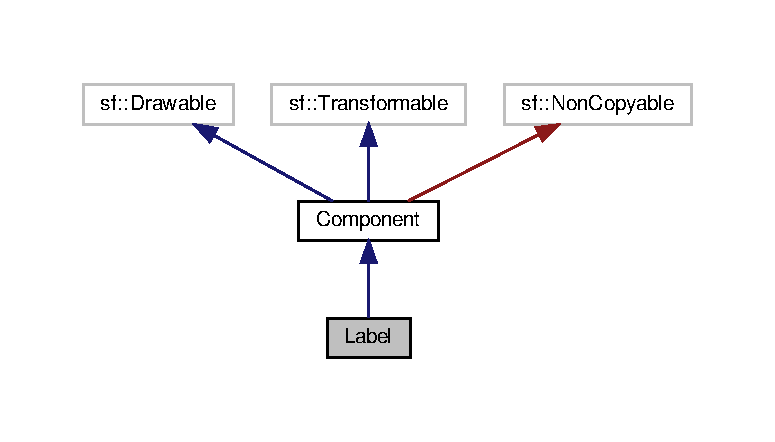
\includegraphics[width=350pt]{classLabel__inherit__graph}
\end{center}
\end{figure}


Collaboration diagram for Label\+:
\nopagebreak
\begin{figure}[H]
\begin{center}
\leavevmode
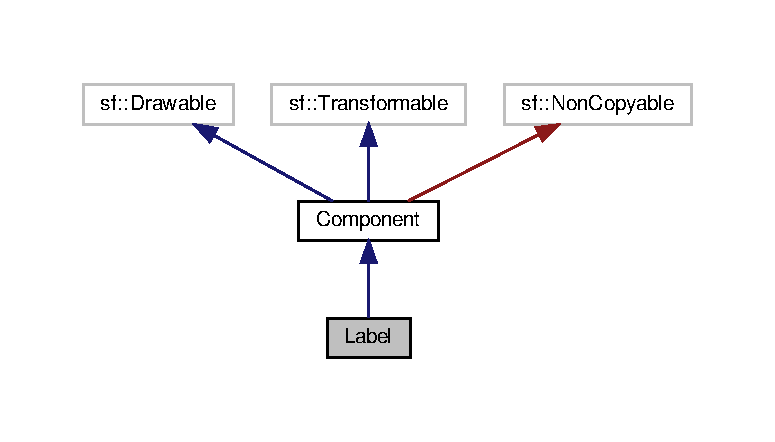
\includegraphics[width=350pt]{classLabel__coll__graph}
\end{center}
\end{figure}
\subsection*{Public Member Functions}
\begin{DoxyCompactItemize}
\item 
\hyperlink{classLabel_ab2454e0a3b79602c481d48f40b5f7a41}{Label} (const std\+::string \&text, const std\+::string \&path, bool \hyperlink{classComponent_aaab29ea159109b4d0f63e9c519be6139}{activate}, float size, bool toogle=false, bool highlighted=false, const sf\+::\+Color color=sf\+::\+Color\+::\+White)
\begin{DoxyCompactList}\small\item\em Construct a new \hyperlink{classLabel}{Label} object, standart constructor, get all the information you need to get it started. \end{DoxyCompactList}\item 
virtual bool \hyperlink{classLabel_ac27e6e31942be4612d282af282b65051}{is\+Selectable} () const
\begin{DoxyCompactList}\small\item\em Open for check-\/in implementations. \end{DoxyCompactList}\item 
void \hyperlink{classLabel_a2bd65842919bc965ff8482407b34f097}{set\+Text} (const std\+::string \&text)
\begin{DoxyCompactList}\small\item\em Set the Text object. \end{DoxyCompactList}\item 
virtual bool \hyperlink{classLabel_a5f1713cf4793b46cf0370ce2d447e722}{update} (sf\+::\+Time dt)
\begin{DoxyCompactList}\small\item\em Responsible for the effects of the texts, such as shining or even appearing with outline. \end{DoxyCompactList}\item 
virtual void \hyperlink{classLabel_a2fd9614a68f0a6b89d3a50316ec4172c}{handle\+Event} (const sf\+::\+Event \&event)
\begin{DoxyCompactList}\small\item\em Here in case you need an implementation. \end{DoxyCompactList}\item 
void \hyperlink{classLabel_ab881215fca0b1450c7c725c333c86220}{set\+Border} (sf\+::\+Color border\+Color, sf\+::\+Color outline, int outline\+Size)
\begin{DoxyCompactList}\small\item\em Set the Border object. \end{DoxyCompactList}\end{DoxyCompactItemize}


\subsection{Detailed Description}
compiles within itself the tools to create a label through S\+F\+ML 

\subsection{Constructor \& Destructor Documentation}
\mbox{\Hypertarget{classLabel_ab2454e0a3b79602c481d48f40b5f7a41}\label{classLabel_ab2454e0a3b79602c481d48f40b5f7a41}} 
\index{Label@{Label}!Label@{Label}}
\index{Label@{Label}!Label@{Label}}
\subsubsection{\texorpdfstring{Label()}{Label()}}
{\footnotesize\ttfamily Label\+::\+Label (\begin{DoxyParamCaption}\item[{const std\+::string \&}]{text,  }\item[{const std\+::string \&}]{path,  }\item[{bool}]{activate,  }\item[{float}]{size,  }\item[{bool}]{toogle = {\ttfamily false},  }\item[{bool}]{highlighted = {\ttfamily false},  }\item[{const sf\+::\+Color}]{color = {\ttfamily sf\+:\+:Color\+:\+:White} }\end{DoxyParamCaption})}



Construct a new \hyperlink{classLabel}{Label} object, standart constructor, get all the information you need to get it started. 


\begin{DoxyParams}{Parameters}
{\em text} & needed into label \\
\hline
{\em path} & font path \\
\hline
{\em activate} & visible or not \\
\hline
{\em size} & text size \\
\hline
{\em toogle} & \\
\hline
{\em highlighted} & \\
\hline
{\em color} & \\
\hline
\end{DoxyParams}


\subsection{Member Function Documentation}
\mbox{\Hypertarget{classLabel_a2fd9614a68f0a6b89d3a50316ec4172c}\label{classLabel_a2fd9614a68f0a6b89d3a50316ec4172c}} 
\index{Label@{Label}!handle\+Event@{handle\+Event}}
\index{handle\+Event@{handle\+Event}!Label@{Label}}
\subsubsection{\texorpdfstring{handle\+Event()}{handleEvent()}}
{\footnotesize\ttfamily void Label\+::handle\+Event (\begin{DoxyParamCaption}\item[{const sf\+::\+Event \&}]{event }\end{DoxyParamCaption})\hspace{0.3cm}{\ttfamily [virtual]}}



Here in case you need an implementation. 


\begin{DoxyParams}{Parameters}
{\em event} & getted action \\
\hline
\end{DoxyParams}


Implements \hyperlink{classComponent}{Component}.

\mbox{\Hypertarget{classLabel_ac27e6e31942be4612d282af282b65051}\label{classLabel_ac27e6e31942be4612d282af282b65051}} 
\index{Label@{Label}!is\+Selectable@{is\+Selectable}}
\index{is\+Selectable@{is\+Selectable}!Label@{Label}}
\subsubsection{\texorpdfstring{is\+Selectable()}{isSelectable()}}
{\footnotesize\ttfamily bool Label\+::is\+Selectable (\begin{DoxyParamCaption}{ }\end{DoxyParamCaption}) const\hspace{0.3cm}{\ttfamily [virtual]}}



Open for check-\/in implementations. 

\begin{DoxyReturn}{Returns}
true 

false 
\end{DoxyReturn}


Implements \hyperlink{classComponent_aede74a18a443413465216f383a046028}{Component}.

\mbox{\Hypertarget{classLabel_ab881215fca0b1450c7c725c333c86220}\label{classLabel_ab881215fca0b1450c7c725c333c86220}} 
\index{Label@{Label}!set\+Border@{set\+Border}}
\index{set\+Border@{set\+Border}!Label@{Label}}
\subsubsection{\texorpdfstring{set\+Border()}{setBorder()}}
{\footnotesize\ttfamily void Label\+::set\+Border (\begin{DoxyParamCaption}\item[{sf\+::\+Color}]{border\+Color,  }\item[{sf\+::\+Color}]{outline,  }\item[{int}]{outline\+Size }\end{DoxyParamCaption})}



Set the Border object. 


\begin{DoxyParams}{Parameters}
{\em border\+Color} & \\
\hline
{\em outline} & \\
\hline
{\em outline\+Size} & \\
\hline
\end{DoxyParams}
\mbox{\Hypertarget{classLabel_a2bd65842919bc965ff8482407b34f097}\label{classLabel_a2bd65842919bc965ff8482407b34f097}} 
\index{Label@{Label}!set\+Text@{set\+Text}}
\index{set\+Text@{set\+Text}!Label@{Label}}
\subsubsection{\texorpdfstring{set\+Text()}{setText()}}
{\footnotesize\ttfamily void Label\+::set\+Text (\begin{DoxyParamCaption}\item[{const std\+::string \&}]{text }\end{DoxyParamCaption})}



Set the Text object. 


\begin{DoxyParams}{Parameters}
{\em text} & \\
\hline
\end{DoxyParams}
\mbox{\Hypertarget{classLabel_a5f1713cf4793b46cf0370ce2d447e722}\label{classLabel_a5f1713cf4793b46cf0370ce2d447e722}} 
\index{Label@{Label}!update@{update}}
\index{update@{update}!Label@{Label}}
\subsubsection{\texorpdfstring{update()}{update()}}
{\footnotesize\ttfamily bool Label\+::update (\begin{DoxyParamCaption}\item[{sf\+::\+Time}]{dt }\end{DoxyParamCaption})\hspace{0.3cm}{\ttfamily [virtual]}}



Responsible for the effects of the texts, such as shining or even appearing with outline. 


\begin{DoxyParams}{Parameters}
{\em dt} & Fraction of time \\
\hline
\end{DoxyParams}
\begin{DoxyReturn}{Returns}
true 

false if have a problem 
\end{DoxyReturn}


Implements \hyperlink{classComponent}{Component}.



The documentation for this class was generated from the following files\+:\begin{DoxyCompactItemize}
\item 
sources/utils/\+Components/Label.\+hpp\item 
sources/utils/\+Components/Label.\+cpp\end{DoxyCompactItemize}

\hypertarget{classMatrix}{}\section{Matrix Class Reference}
\label{classMatrix}\index{Matrix@{Matrix}}
\subsection*{Public Member Functions}
\begin{DoxyCompactItemize}
\item 
bool \hyperlink{classMatrix_a2f7248b95312e5ecabeab518cd584774}{tetromino\+Compatible} (std\+::vector$<$ sf\+::\+Vector2i $>$ pos)
\begin{DoxyCompactList}\small\item\em Check all the board positions according to the next positions to check if it is possible to fit the piece. \end{DoxyCompactList}\item 
int \hyperlink{classMatrix_ac4c14902c7108f0f9ac46ee9d1ef92f9}{code\+Position} (int x, int y)
\begin{DoxyCompactList}\small\item\em Encodes received coordinates; from 2D to 1D. \end{DoxyCompactList}\item 
sf\+::\+Vector2i \hyperlink{classMatrix_a5680e2198758d4b7524810d0e0fe4021}{decode\+Position} (int code)
\begin{DoxyCompactList}\small\item\em Retrieves the coded message from one dimension to two dimensions. \end{DoxyCompactList}\item 
int \hyperlink{classMatrix_a3f51ba6280305f2d692ab754800297fa}{get\+Width} ()
\begin{DoxyCompactList}\small\item\em Get the Width object. \end{DoxyCompactList}\item 
int \hyperlink{classMatrix_a3af39c453aeb30c5cb55f72c2e71917f}{get\+Height} ()
\begin{DoxyCompactList}\small\item\em Get the Height object. \end{DoxyCompactList}\item 
std\+::vector$<$ int $>$ \hyperlink{classMatrix_a9fa09bc31e6e2dfe4ced74eb34de0f70}{get\+Pos} () const
\begin{DoxyCompactList}\small\item\em Get the Pos object in relation to the two coordinates of the matrix. \end{DoxyCompactList}\item 
\mbox{\Hypertarget{classMatrix_a765f4dcb51b6829311cc3e7576388423}\label{classMatrix_a765f4dcb51b6829311cc3e7576388423}} 
{\bfseries Matrix} (const \hyperlink{classMatrix}{Matrix} \&m)
\item 
\mbox{\Hypertarget{classMatrix_a5d5b33d74cf6443d9c2b6242b3f7e320}\label{classMatrix_a5d5b33d74cf6443d9c2b6242b3f7e320}} 
{\bfseries Matrix} (int width, int height)
\item 
bool \hyperlink{classMatrix_a993ef93c4c0b32047586dd3e3a981853}{operator==} (\hyperlink{classTetromino}{Tetromino} \&t)
\begin{DoxyCompactList}\small\item\em It directly compares a tetromino with the place where it will be to place it. \end{DoxyCompactList}\item 
int \hyperlink{classMatrix_abd7645de0cb39d103a96c0f905a1cebe}{update\+Lines} (\hyperlink{classTetromino}{Tetromino} t)
\begin{DoxyCompactList}\small\item\em Checks the lines to update according to the parts that are already positioned inside the matrix. \end{DoxyCompactList}\item 
\mbox{\Hypertarget{classMatrix_abb14e34d409ecd4133c2840755b556b7}\label{classMatrix_abb14e34d409ecd4133c2840755b556b7}} 
void \hyperlink{classMatrix_abb14e34d409ecd4133c2840755b556b7}{restart} ()
\begin{DoxyCompactList}\small\item\em Reset \hyperlink{classMatrix}{Matrix}. \end{DoxyCompactList}\end{DoxyCompactItemize}
\subsection*{Friends}
\begin{DoxyCompactItemize}
\item 
\hyperlink{classMatrix}{Matrix} \& \hyperlink{classMatrix_ac1bb2cc60467d7aaa22c10217f500ec9}{operator+} (\hyperlink{classMatrix}{Matrix} m, \hyperlink{classTetromino}{Tetromino} \&t)
\begin{DoxyCompactList}\small\item\em Moves the part in the axis and making the movement of the tetromino simpler. \end{DoxyCompactList}\item 
\mbox{\Hypertarget{classMatrix_ae94f48053f851e77e8f461e5ab1e3fdd}\label{classMatrix_ae94f48053f851e77e8f461e5ab1e3fdd}} 
std\+::ostream \& {\bfseries operator$<$$<$} (std\+::ostream \&o, \hyperlink{classMatrix}{Matrix} \&m)
\end{DoxyCompactItemize}


\subsection{Member Function Documentation}
\mbox{\Hypertarget{classMatrix_ac4c14902c7108f0f9ac46ee9d1ef92f9}\label{classMatrix_ac4c14902c7108f0f9ac46ee9d1ef92f9}} 
\index{Matrix@{Matrix}!code\+Position@{code\+Position}}
\index{code\+Position@{code\+Position}!Matrix@{Matrix}}
\subsubsection{\texorpdfstring{code\+Position()}{codePosition()}}
{\footnotesize\ttfamily int Matrix\+::code\+Position (\begin{DoxyParamCaption}\item[{int}]{x,  }\item[{int}]{y }\end{DoxyParamCaption})}



Encodes received coordinates; from 2D to 1D. 


\begin{DoxyParams}{Parameters}
{\em x} & Position value \\
\hline
{\em y} & Position value \\
\hline
\end{DoxyParams}
\begin{DoxyReturn}{Returns}
The coding 
\end{DoxyReturn}
\mbox{\Hypertarget{classMatrix_a5680e2198758d4b7524810d0e0fe4021}\label{classMatrix_a5680e2198758d4b7524810d0e0fe4021}} 
\index{Matrix@{Matrix}!decode\+Position@{decode\+Position}}
\index{decode\+Position@{decode\+Position}!Matrix@{Matrix}}
\subsubsection{\texorpdfstring{decode\+Position()}{decodePosition()}}
{\footnotesize\ttfamily sf\+::\+Vector2i Matrix\+::decode\+Position (\begin{DoxyParamCaption}\item[{int}]{code }\end{DoxyParamCaption})}



Retrieves the coded message from one dimension to two dimensions. 


\begin{DoxyParams}{Parameters}
{\em code} & in 1D \\
\hline
\end{DoxyParams}
\begin{DoxyReturn}{Returns}
sf\+::\+Vector2i with 2D 
\end{DoxyReturn}
\mbox{\Hypertarget{classMatrix_a3af39c453aeb30c5cb55f72c2e71917f}\label{classMatrix_a3af39c453aeb30c5cb55f72c2e71917f}} 
\index{Matrix@{Matrix}!get\+Height@{get\+Height}}
\index{get\+Height@{get\+Height}!Matrix@{Matrix}}
\subsubsection{\texorpdfstring{get\+Height()}{getHeight()}}
{\footnotesize\ttfamily int Matrix\+::get\+Height (\begin{DoxyParamCaption}{ }\end{DoxyParamCaption})}



Get the Height object. 

\begin{DoxyReturn}{Returns}
int value 
\end{DoxyReturn}
\mbox{\Hypertarget{classMatrix_a9fa09bc31e6e2dfe4ced74eb34de0f70}\label{classMatrix_a9fa09bc31e6e2dfe4ced74eb34de0f70}} 
\index{Matrix@{Matrix}!get\+Pos@{get\+Pos}}
\index{get\+Pos@{get\+Pos}!Matrix@{Matrix}}
\subsubsection{\texorpdfstring{get\+Pos()}{getPos()}}
{\footnotesize\ttfamily std\+::vector$<$ int $>$ Matrix\+::get\+Pos (\begin{DoxyParamCaption}{ }\end{DoxyParamCaption}) const}



Get the Pos object in relation to the two coordinates of the matrix. 

\begin{DoxyReturn}{Returns}
std\+::vector$<$int$>$ 
\end{DoxyReturn}
\mbox{\Hypertarget{classMatrix_a3f51ba6280305f2d692ab754800297fa}\label{classMatrix_a3f51ba6280305f2d692ab754800297fa}} 
\index{Matrix@{Matrix}!get\+Width@{get\+Width}}
\index{get\+Width@{get\+Width}!Matrix@{Matrix}}
\subsubsection{\texorpdfstring{get\+Width()}{getWidth()}}
{\footnotesize\ttfamily int Matrix\+::get\+Width (\begin{DoxyParamCaption}{ }\end{DoxyParamCaption})}



Get the Width object. 

\begin{DoxyReturn}{Returns}
int value 
\end{DoxyReturn}
\mbox{\Hypertarget{classMatrix_a993ef93c4c0b32047586dd3e3a981853}\label{classMatrix_a993ef93c4c0b32047586dd3e3a981853}} 
\index{Matrix@{Matrix}!operator==@{operator==}}
\index{operator==@{operator==}!Matrix@{Matrix}}
\subsubsection{\texorpdfstring{operator==()}{operator==()}}
{\footnotesize\ttfamily bool Matrix\+::operator== (\begin{DoxyParamCaption}\item[{\hyperlink{classTetromino}{Tetromino} \&}]{t }\end{DoxyParamCaption})}



It directly compares a tetromino with the place where it will be to place it. 


\begin{DoxyParams}{Parameters}
{\em t} & \hyperlink{classTetromino}{Tetromino} getted for comparation \\
\hline
\end{DoxyParams}
\begin{DoxyReturn}{Returns}
true 

false 
\end{DoxyReturn}
\mbox{\Hypertarget{classMatrix_a2f7248b95312e5ecabeab518cd584774}\label{classMatrix_a2f7248b95312e5ecabeab518cd584774}} 
\index{Matrix@{Matrix}!tetromino\+Compatible@{tetromino\+Compatible}}
\index{tetromino\+Compatible@{tetromino\+Compatible}!Matrix@{Matrix}}
\subsubsection{\texorpdfstring{tetromino\+Compatible()}{tetrominoCompatible()}}
{\footnotesize\ttfamily bool Matrix\+::tetromino\+Compatible (\begin{DoxyParamCaption}\item[{std\+::vector$<$ sf\+::\+Vector2i $>$}]{pos }\end{DoxyParamCaption})}



Check all the board positions according to the next positions to check if it is possible to fit the piece. 


\begin{DoxyParams}{Parameters}
{\em pos} & \\
\hline
\end{DoxyParams}
\begin{DoxyReturn}{Returns}
true 

false if it is not possible to fit the piece 
\end{DoxyReturn}
\mbox{\Hypertarget{classMatrix_abd7645de0cb39d103a96c0f905a1cebe}\label{classMatrix_abd7645de0cb39d103a96c0f905a1cebe}} 
\index{Matrix@{Matrix}!update\+Lines@{update\+Lines}}
\index{update\+Lines@{update\+Lines}!Matrix@{Matrix}}
\subsubsection{\texorpdfstring{update\+Lines()}{updateLines()}}
{\footnotesize\ttfamily int Matrix\+::update\+Lines (\begin{DoxyParamCaption}\item[{\hyperlink{classTetromino}{Tetromino}}]{t }\end{DoxyParamCaption})}



Checks the lines to update according to the parts that are already positioned inside the matrix. 


\begin{DoxyParams}{Parameters}
{\em t} & positions of tetromino \\
\hline
\end{DoxyParams}
\begin{DoxyReturn}{Returns}
int 
\end{DoxyReturn}


\subsection{Friends And Related Function Documentation}
\mbox{\Hypertarget{classMatrix_ac1bb2cc60467d7aaa22c10217f500ec9}\label{classMatrix_ac1bb2cc60467d7aaa22c10217f500ec9}} 
\index{Matrix@{Matrix}!operator+@{operator+}}
\index{operator+@{operator+}!Matrix@{Matrix}}
\subsubsection{\texorpdfstring{operator+}{operator+}}
{\footnotesize\ttfamily \hyperlink{classMatrix}{Matrix}\& operator+ (\begin{DoxyParamCaption}\item[{\hyperlink{classMatrix}{Matrix}}]{m,  }\item[{\hyperlink{classTetromino}{Tetromino} \&}]{t }\end{DoxyParamCaption})\hspace{0.3cm}{\ttfamily [friend]}}



Moves the part in the axis and making the movement of the tetromino simpler. 


\begin{DoxyParams}{Parameters}
{\em m} & Base \hyperlink{classMatrix}{Matrix} \\
\hline
{\em t} & tetromino for comparation \\
\hline
\end{DoxyParams}
\begin{DoxyReturn}{Returns}
\hyperlink{classMatrix}{Matrix}\& 
\end{DoxyReturn}


The documentation for this class was generated from the following files\+:\begin{DoxyCompactItemize}
\item 
sources/game/Matrix.\+hpp\item 
sources/game/Matrix.\+cpp\end{DoxyCompactItemize}

\hypertarget{classMenuScene}{}\section{Menu\+Scene Class Reference}
\label{classMenuScene}\index{Menu\+Scene@{Menu\+Scene}}


responsible for viewing the game\textquotesingle{}s main menu  




{\ttfamily \#include $<$Menu\+Scene.\+hpp$>$}



Inheritance diagram for Menu\+Scene\+:
\nopagebreak
\begin{figure}[H]
\begin{center}
\leavevmode
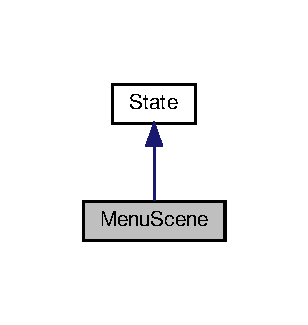
\includegraphics[width=148pt]{classMenuScene__inherit__graph}
\end{center}
\end{figure}


Collaboration diagram for Menu\+Scene\+:
\nopagebreak
\begin{figure}[H]
\begin{center}
\leavevmode
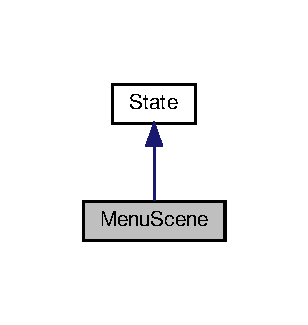
\includegraphics[width=148pt]{classMenuScene__coll__graph}
\end{center}
\end{figure}
\subsection*{Public Member Functions}
\begin{DoxyCompactItemize}
\item 
\hyperlink{classMenuScene_ad5964f15d3a3f9daa3ab89c8cb4eb3b6}{Menu\+Scene} (\hyperlink{classStateManager}{State\+Manager} \&stack, \hyperlink{structState_1_1Context}{Context} context)
\begin{DoxyCompactList}\small\item\em Construct a new Menu Scene object, standard builder. \end{DoxyCompactList}\item 
\mbox{\Hypertarget{classMenuScene_a1950514cb59988544094f4a18feef437}\label{classMenuScene_a1950514cb59988544094f4a18feef437}} 
virtual void \hyperlink{classMenuScene_a1950514cb59988544094f4a18feef437}{draw} ()
\begin{DoxyCompactList}\small\item\em overwriting the function drawing by adding new elements responsible for sampling new elements added to this view \end{DoxyCompactList}\item 
virtual bool \hyperlink{classMenuScene_ab18847a026d82d5ffe8c869bbf78725e}{update} (sf\+::\+Time dt)
\begin{DoxyCompactList}\small\item\em overwriting the function update by adding new elements responsible for sampling new elements added to this view \end{DoxyCompactList}\item 
virtual bool \hyperlink{classMenuScene_a47f06ae8b2a4830a0a6d104db52fd624}{handle\+Event} (const sf\+::\+Event \&event)
\begin{DoxyCompactList}\small\item\em Adds new features to the function responsible for handling the events, adding a specific function for each key depending on the view. \end{DoxyCompactList}\end{DoxyCompactItemize}
\subsection*{Additional Inherited Members}


\subsection{Detailed Description}
responsible for viewing the game\textquotesingle{}s main menu 

\subsection{Constructor \& Destructor Documentation}
\mbox{\Hypertarget{classMenuScene_ad5964f15d3a3f9daa3ab89c8cb4eb3b6}\label{classMenuScene_ad5964f15d3a3f9daa3ab89c8cb4eb3b6}} 
\index{Menu\+Scene@{Menu\+Scene}!Menu\+Scene@{Menu\+Scene}}
\index{Menu\+Scene@{Menu\+Scene}!Menu\+Scene@{Menu\+Scene}}
\subsubsection{\texorpdfstring{Menu\+Scene()}{MenuScene()}}
{\footnotesize\ttfamily Menu\+Scene\+::\+Menu\+Scene (\begin{DoxyParamCaption}\item[{\hyperlink{classStateManager}{State\+Manager} \&}]{stack,  }\item[{\hyperlink{structState_1_1Context}{Context}}]{context }\end{DoxyParamCaption})}



Construct a new Menu Scene object, standard builder. 


\begin{DoxyParams}{Parameters}
{\em stack} & stack responsible for managing the views \\
\hline
{\em context} & relates all current context \\
\hline
\end{DoxyParams}


\subsection{Member Function Documentation}
\mbox{\Hypertarget{classMenuScene_a47f06ae8b2a4830a0a6d104db52fd624}\label{classMenuScene_a47f06ae8b2a4830a0a6d104db52fd624}} 
\index{Menu\+Scene@{Menu\+Scene}!handle\+Event@{handle\+Event}}
\index{handle\+Event@{handle\+Event}!Menu\+Scene@{Menu\+Scene}}
\subsubsection{\texorpdfstring{handle\+Event()}{handleEvent()}}
{\footnotesize\ttfamily bool Menu\+Scene\+::handle\+Event (\begin{DoxyParamCaption}\item[{const sf\+::\+Event \&}]{event }\end{DoxyParamCaption})\hspace{0.3cm}{\ttfamily [virtual]}}



Adds new features to the function responsible for handling the events, adding a specific function for each key depending on the view. 


\begin{DoxyParams}{Parameters}
{\em event} & getted action \\
\hline
\end{DoxyParams}
\begin{DoxyReturn}{Returns}
true 

false if have a problem 
\end{DoxyReturn}


Implements \hyperlink{classState_a19965f83460b248c42952aac8d001206}{State}.

\mbox{\Hypertarget{classMenuScene_ab18847a026d82d5ffe8c869bbf78725e}\label{classMenuScene_ab18847a026d82d5ffe8c869bbf78725e}} 
\index{Menu\+Scene@{Menu\+Scene}!update@{update}}
\index{update@{update}!Menu\+Scene@{Menu\+Scene}}
\subsubsection{\texorpdfstring{update()}{update()}}
{\footnotesize\ttfamily bool Menu\+Scene\+::update (\begin{DoxyParamCaption}\item[{sf\+::\+Time}]{dt }\end{DoxyParamCaption})\hspace{0.3cm}{\ttfamily [virtual]}}



overwriting the function update by adding new elements responsible for sampling new elements added to this view 


\begin{DoxyParams}{Parameters}
{\em dt} & Fraction of time \\
\hline
\end{DoxyParams}
\begin{DoxyReturn}{Returns}
true 

false if have a problem 
\end{DoxyReturn}


Implements \hyperlink{classState_acd5926bc7a373edff9e57f3ffe94ca13}{State}.



The documentation for this class was generated from the following files\+:\begin{DoxyCompactItemize}
\item 
sources/views/Menu\+Scene.\+hpp\item 
sources/views/Menu\+Scene.\+cpp\end{DoxyCompactItemize}

\hypertarget{classMultiplayerScene}{}\section{Multiplayer\+Scene Class Reference}
\label{classMultiplayerScene}\index{Multiplayer\+Scene@{Multiplayer\+Scene}}


class responsible for taking care of the introduction Multiplayer screen of the game  




{\ttfamily \#include $<$Multiplayer\+Scene.\+hpp$>$}



Inheritance diagram for Multiplayer\+Scene\+:
\nopagebreak
\begin{figure}[H]
\begin{center}
\leavevmode
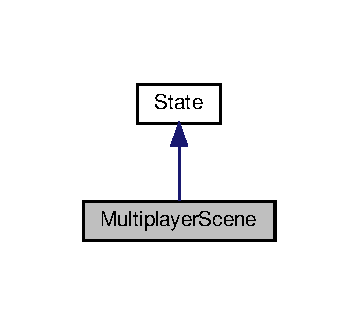
\includegraphics[width=172pt]{classMultiplayerScene__inherit__graph}
\end{center}
\end{figure}


Collaboration diagram for Multiplayer\+Scene\+:
\nopagebreak
\begin{figure}[H]
\begin{center}
\leavevmode
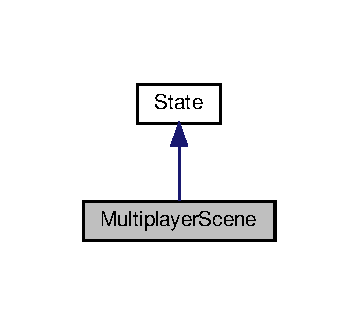
\includegraphics[width=172pt]{classMultiplayerScene__coll__graph}
\end{center}
\end{figure}
\subsection*{Public Member Functions}
\begin{DoxyCompactItemize}
\item 
\hyperlink{classMultiplayerScene_a0a555300aaf7b66d983e35c8b6dbe495}{Multiplayer\+Scene} (\hyperlink{classStateManager}{State\+Manager} \&stack, \hyperlink{structState_1_1Context}{Context} context)
\begin{DoxyCompactList}\small\item\em Construct a new Multiplayer Scene object, standard builder. \end{DoxyCompactList}\item 
\mbox{\Hypertarget{classMultiplayerScene_ad6398a29ef541078c1697f043ed53fbe}\label{classMultiplayerScene_ad6398a29ef541078c1697f043ed53fbe}} 
virtual void \hyperlink{classMultiplayerScene_ad6398a29ef541078c1697f043ed53fbe}{draw} ()
\begin{DoxyCompactList}\small\item\em overwriting the function drawing by adding new elements responsible for sampling new elements added to this view \end{DoxyCompactList}\item 
virtual bool \hyperlink{classMultiplayerScene_a7d55178de89a4de08bdd1aaa7561756e}{update} (sf\+::\+Time dt)
\begin{DoxyCompactList}\small\item\em overwriting the function update by adding new elements responsible for sampling new elements added to this view \end{DoxyCompactList}\item 
virtual bool \hyperlink{classMultiplayerScene_af2bcc458cda1d272acabc342eb79d25a}{handle\+Event} (const sf\+::\+Event \&event)
\begin{DoxyCompactList}\small\item\em Adds new features to the function responsible for handling the events, adding a specific function for each key depending on the view. \end{DoxyCompactList}\item 
void \hyperlink{classMultiplayerScene_afec1f9d6c9cf3e1bc9d6a2485bd4ed46}{handle\+Multiplayer} (bool create\+Connection)
\begin{DoxyCompactList}\small\item\em Responsible for making message settings and calling up connection functions. \end{DoxyCompactList}\end{DoxyCompactItemize}
\subsection*{Additional Inherited Members}


\subsection{Detailed Description}
class responsible for taking care of the introduction Multiplayer screen of the game 

\subsection{Constructor \& Destructor Documentation}
\mbox{\Hypertarget{classMultiplayerScene_a0a555300aaf7b66d983e35c8b6dbe495}\label{classMultiplayerScene_a0a555300aaf7b66d983e35c8b6dbe495}} 
\index{Multiplayer\+Scene@{Multiplayer\+Scene}!Multiplayer\+Scene@{Multiplayer\+Scene}}
\index{Multiplayer\+Scene@{Multiplayer\+Scene}!Multiplayer\+Scene@{Multiplayer\+Scene}}
\subsubsection{\texorpdfstring{Multiplayer\+Scene()}{MultiplayerScene()}}
{\footnotesize\ttfamily Multiplayer\+Scene\+::\+Multiplayer\+Scene (\begin{DoxyParamCaption}\item[{\hyperlink{classStateManager}{State\+Manager} \&}]{stack,  }\item[{\hyperlink{structState_1_1Context}{Context}}]{context }\end{DoxyParamCaption})}



Construct a new Multiplayer Scene object, standard builder. 


\begin{DoxyParams}{Parameters}
{\em stack} & stack responsible for managing the views \\
\hline
{\em context} & relates all current context \\
\hline
\end{DoxyParams}


\subsection{Member Function Documentation}
\mbox{\Hypertarget{classMultiplayerScene_af2bcc458cda1d272acabc342eb79d25a}\label{classMultiplayerScene_af2bcc458cda1d272acabc342eb79d25a}} 
\index{Multiplayer\+Scene@{Multiplayer\+Scene}!handle\+Event@{handle\+Event}}
\index{handle\+Event@{handle\+Event}!Multiplayer\+Scene@{Multiplayer\+Scene}}
\subsubsection{\texorpdfstring{handle\+Event()}{handleEvent()}}
{\footnotesize\ttfamily bool Multiplayer\+Scene\+::handle\+Event (\begin{DoxyParamCaption}\item[{const sf\+::\+Event \&}]{event }\end{DoxyParamCaption})\hspace{0.3cm}{\ttfamily [virtual]}}



Adds new features to the function responsible for handling the events, adding a specific function for each key depending on the view. 


\begin{DoxyParams}{Parameters}
{\em event} & getted action \\
\hline
\end{DoxyParams}
\begin{DoxyReturn}{Returns}
true 

false if have a problem 
\end{DoxyReturn}


Implements \hyperlink{classState_a19965f83460b248c42952aac8d001206}{State}.

\mbox{\Hypertarget{classMultiplayerScene_afec1f9d6c9cf3e1bc9d6a2485bd4ed46}\label{classMultiplayerScene_afec1f9d6c9cf3e1bc9d6a2485bd4ed46}} 
\index{Multiplayer\+Scene@{Multiplayer\+Scene}!handle\+Multiplayer@{handle\+Multiplayer}}
\index{handle\+Multiplayer@{handle\+Multiplayer}!Multiplayer\+Scene@{Multiplayer\+Scene}}
\subsubsection{\texorpdfstring{handle\+Multiplayer()}{handleMultiplayer()}}
{\footnotesize\ttfamily void Multiplayer\+Scene\+::handle\+Multiplayer (\begin{DoxyParamCaption}\item[{bool}]{create\+Connection }\end{DoxyParamCaption})}



Responsible for making message settings and calling up connection functions. 


\begin{DoxyParams}{Parameters}
{\em create\+Connection} & defines the action to be taken \\
\hline
\end{DoxyParams}
\mbox{\Hypertarget{classMultiplayerScene_a7d55178de89a4de08bdd1aaa7561756e}\label{classMultiplayerScene_a7d55178de89a4de08bdd1aaa7561756e}} 
\index{Multiplayer\+Scene@{Multiplayer\+Scene}!update@{update}}
\index{update@{update}!Multiplayer\+Scene@{Multiplayer\+Scene}}
\subsubsection{\texorpdfstring{update()}{update()}}
{\footnotesize\ttfamily bool Multiplayer\+Scene\+::update (\begin{DoxyParamCaption}\item[{sf\+::\+Time}]{dt }\end{DoxyParamCaption})\hspace{0.3cm}{\ttfamily [virtual]}}



overwriting the function update by adding new elements responsible for sampling new elements added to this view 


\begin{DoxyParams}{Parameters}
{\em dt} & Fraction of time \\
\hline
\end{DoxyParams}
\begin{DoxyReturn}{Returns}
true 

false if have a problem 
\end{DoxyReturn}


Implements \hyperlink{classState_acd5926bc7a373edff9e57f3ffe94ca13}{State}.



The documentation for this class was generated from the following files\+:\begin{DoxyCompactItemize}
\item 
sources/views/Multiplayer\+Scene.\+hpp\item 
sources/views/Multiplayer\+Scene.\+cpp\end{DoxyCompactItemize}

\hypertarget{classPauseScene}{}\section{Pause\+Scene Class Reference}
\label{classPauseScene}\index{Pause\+Scene@{Pause\+Scene}}


Inheritance diagram for Pause\+Scene\+:
\nopagebreak
\begin{figure}[H]
\begin{center}
\leavevmode
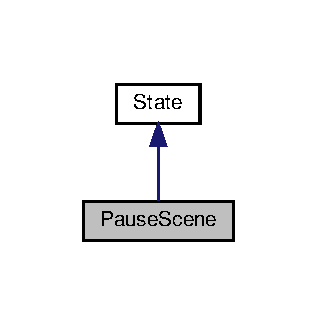
\includegraphics[width=152pt]{classPauseScene__inherit__graph}
\end{center}
\end{figure}


Collaboration diagram for Pause\+Scene\+:
\nopagebreak
\begin{figure}[H]
\begin{center}
\leavevmode
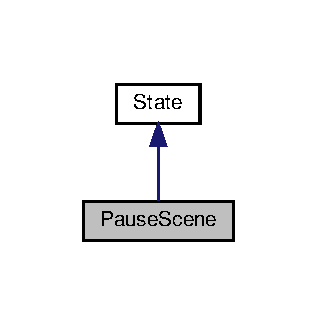
\includegraphics[width=152pt]{classPauseScene__coll__graph}
\end{center}
\end{figure}
\subsection*{Public Member Functions}
\begin{DoxyCompactItemize}
\item 
\hyperlink{classPauseScene_ac9713bd8685f2d6793d8b5379c0e8aa6}{Pause\+Scene} (\hyperlink{classStateManager}{State\+Manager} \&stack, \hyperlink{structState_1_1Context}{Context} context)
\begin{DoxyCompactList}\small\item\em Construct a new Menu Scene object, standard builder. \end{DoxyCompactList}\item 
\mbox{\Hypertarget{classPauseScene_a2f62c5525c35fdc95420418e8b78995f}\label{classPauseScene_a2f62c5525c35fdc95420418e8b78995f}} 
virtual void \hyperlink{classPauseScene_a2f62c5525c35fdc95420418e8b78995f}{draw} ()
\begin{DoxyCompactList}\small\item\em overwriting the function drawing by adding new elements responsible for sampling new elements added to this view \end{DoxyCompactList}\item 
virtual bool \hyperlink{classPauseScene_ab1d5af95abe16f5d7a0cd98b9d1e1c96}{update} (sf\+::\+Time dt)
\begin{DoxyCompactList}\small\item\em overwriting the function update by adding new elements responsible for sampling new elements added to this view \end{DoxyCompactList}\item 
virtual bool \hyperlink{classPauseScene_ad806125bd5ae985f24ff2cbfffc2c8e7}{handle\+Event} (const sf\+::\+Event \&event)
\begin{DoxyCompactList}\small\item\em Adds new features to the function responsible for handling the events, adding a specific function for each key depending on the view. \end{DoxyCompactList}\end{DoxyCompactItemize}
\subsection*{Additional Inherited Members}


\subsection{Constructor \& Destructor Documentation}
\mbox{\Hypertarget{classPauseScene_ac9713bd8685f2d6793d8b5379c0e8aa6}\label{classPauseScene_ac9713bd8685f2d6793d8b5379c0e8aa6}} 
\index{Pause\+Scene@{Pause\+Scene}!Pause\+Scene@{Pause\+Scene}}
\index{Pause\+Scene@{Pause\+Scene}!Pause\+Scene@{Pause\+Scene}}
\subsubsection{\texorpdfstring{Pause\+Scene()}{PauseScene()}}
{\footnotesize\ttfamily Pause\+Scene\+::\+Pause\+Scene (\begin{DoxyParamCaption}\item[{\hyperlink{classStateManager}{State\+Manager} \&}]{stack,  }\item[{\hyperlink{structState_1_1Context}{Context}}]{context }\end{DoxyParamCaption})}



Construct a new Menu Scene object, standard builder. 


\begin{DoxyParams}{Parameters}
{\em stack} & stack responsible for managing the views \\
\hline
{\em context} & relates all current context \\
\hline
\end{DoxyParams}


\subsection{Member Function Documentation}
\mbox{\Hypertarget{classPauseScene_ad806125bd5ae985f24ff2cbfffc2c8e7}\label{classPauseScene_ad806125bd5ae985f24ff2cbfffc2c8e7}} 
\index{Pause\+Scene@{Pause\+Scene}!handle\+Event@{handle\+Event}}
\index{handle\+Event@{handle\+Event}!Pause\+Scene@{Pause\+Scene}}
\subsubsection{\texorpdfstring{handle\+Event()}{handleEvent()}}
{\footnotesize\ttfamily bool Pause\+Scene\+::handle\+Event (\begin{DoxyParamCaption}\item[{const sf\+::\+Event \&}]{event }\end{DoxyParamCaption})\hspace{0.3cm}{\ttfamily [virtual]}}



Adds new features to the function responsible for handling the events, adding a specific function for each key depending on the view. 


\begin{DoxyParams}{Parameters}
{\em event} & getted action \\
\hline
\end{DoxyParams}
\begin{DoxyReturn}{Returns}
true 

false if have a problem 
\end{DoxyReturn}


Implements \hyperlink{classState_a19965f83460b248c42952aac8d001206}{State}.

\mbox{\Hypertarget{classPauseScene_ab1d5af95abe16f5d7a0cd98b9d1e1c96}\label{classPauseScene_ab1d5af95abe16f5d7a0cd98b9d1e1c96}} 
\index{Pause\+Scene@{Pause\+Scene}!update@{update}}
\index{update@{update}!Pause\+Scene@{Pause\+Scene}}
\subsubsection{\texorpdfstring{update()}{update()}}
{\footnotesize\ttfamily bool Pause\+Scene\+::update (\begin{DoxyParamCaption}\item[{sf\+::\+Time}]{dt }\end{DoxyParamCaption})\hspace{0.3cm}{\ttfamily [virtual]}}



overwriting the function update by adding new elements responsible for sampling new elements added to this view 


\begin{DoxyParams}{Parameters}
{\em dt} & Fraction of time \\
\hline
\end{DoxyParams}
\begin{DoxyReturn}{Returns}
true 

false if have a problem 
\end{DoxyReturn}


Implements \hyperlink{classState_acd5926bc7a373edff9e57f3ffe94ca13}{State}.



The documentation for this class was generated from the following files\+:\begin{DoxyCompactItemize}
\item 
sources/views/Pause\+Scene.\+hpp\item 
sources/views/Pause\+Scene.\+cpp\end{DoxyCompactItemize}

\hypertarget{classPlayer}{}\section{Player Class Reference}
\label{classPlayer}\index{Player@{Player}}
\subsection*{Public Member Functions}
\begin{DoxyCompactItemize}
\item 
\mbox{\Hypertarget{classPlayer_a555e879c595e8b0fd6aa115981ca52de}\label{classPlayer_a555e879c595e8b0fd6aa115981ca52de}} 
{\bfseries Player} (bool pause, int score, int level)
\item 
\mbox{\Hypertarget{classPlayer_a133cd7426d3d94be3d6206248a368a05}\label{classPlayer_a133cd7426d3d94be3d6206248a368a05}} 
bool {\bfseries get\+Pause} ()
\item 
\mbox{\Hypertarget{classPlayer_a97e5447778ae6c384eedc532dcd8431d}\label{classPlayer_a97e5447778ae6c384eedc532dcd8431d}} 
int {\bfseries get\+Score} ()
\item 
\mbox{\Hypertarget{classPlayer_a10dad3b41b420fcc88e83370d981d35b}\label{classPlayer_a10dad3b41b420fcc88e83370d981d35b}} 
int {\bfseries get\+Level} ()
\item 
\mbox{\Hypertarget{classPlayer_ad6aeca23f071b27bd128bd855a54304e}\label{classPlayer_ad6aeca23f071b27bd128bd855a54304e}} 
int {\bfseries get\+Restart} ()
\item 
\mbox{\Hypertarget{classPlayer_a232a2b887a487cf34397509ee6717846}\label{classPlayer_a232a2b887a487cf34397509ee6717846}} 
int {\bfseries get\+Multiplayer} ()
\item 
\mbox{\Hypertarget{classPlayer_a4c5b1bc0955ff4cac217d2a073bb022f}\label{classPlayer_a4c5b1bc0955ff4cac217d2a073bb022f}} 
void {\bfseries set\+Restart} (bool pause)
\item 
\mbox{\Hypertarget{classPlayer_a1dd7a7ed463a04131e6a61b6f8062b8b}\label{classPlayer_a1dd7a7ed463a04131e6a61b6f8062b8b}} 
void {\bfseries set\+Multiplayer} (bool score)
\item 
\mbox{\Hypertarget{classPlayer_a03466eb73d7d9ea95c1b0f9798624961}\label{classPlayer_a03466eb73d7d9ea95c1b0f9798624961}} 
void {\bfseries set\+Pause} (bool pause)
\item 
\mbox{\Hypertarget{classPlayer_a23c9b25aeb8dd1ff86d03d993e07a73d}\label{classPlayer_a23c9b25aeb8dd1ff86d03d993e07a73d}} 
void {\bfseries set\+Score} (int score)
\item 
\mbox{\Hypertarget{classPlayer_af717f3bf17090888a9d504d3919d62cd}\label{classPlayer_af717f3bf17090888a9d504d3919d62cd}} 
void {\bfseries set\+Level} (int level)
\item 
\mbox{\Hypertarget{classPlayer_a3a573dd4bf5e1d241684a0eea064461c}\label{classPlayer_a3a573dd4bf5e1d241684a0eea064461c}} 
void {\bfseries establish\+Connection} (bool create)
\item 
\mbox{\Hypertarget{classPlayer_a28cf39bcf811455210045ced3eeb73da}\label{classPlayer_a28cf39bcf811455210045ced3eeb73da}} 
void {\bfseries establish\+Role} (bool create)
\item 
\mbox{\Hypertarget{classPlayer_aec43cf0af5b0b2dec1facb35a407f975}\label{classPlayer_aec43cf0af5b0b2dec1facb35a407f975}} 
void {\bfseries recv\+Data} (std\+::vector$<$ int $>$ \&v)
\item 
\mbox{\Hypertarget{classPlayer_aeb26fb2ea26e531208d1c8d1e22115a3}\label{classPlayer_aeb26fb2ea26e531208d1c8d1e22115a3}} 
void {\bfseries send\+Data} (std\+::vector$<$ int $>$ v)
\end{DoxyCompactItemize}


The documentation for this class was generated from the following files\+:\begin{DoxyCompactItemize}
\item 
sources/utils/Player.\+hpp\item 
sources/utils/Player.\+cpp\end{DoxyCompactItemize}

\hypertarget{classState}{}\section{State Class Reference}
\label{classState}\index{State@{State}}


Inheritance diagram for State\+:
\nopagebreak
\begin{figure}[H]
\begin{center}
\leavevmode
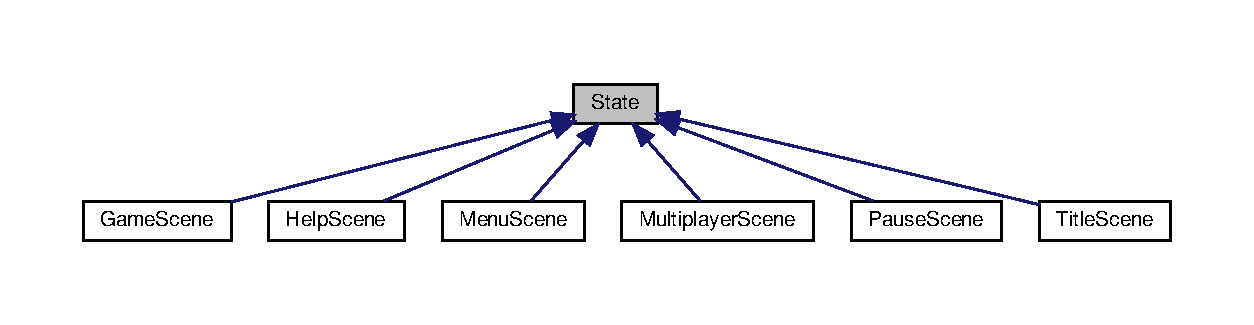
\includegraphics[width=350pt]{classState__inherit__graph}
\end{center}
\end{figure}
\subsection*{Classes}
\begin{DoxyCompactItemize}
\item 
struct \hyperlink{structState_1_1Context}{Context}
\begin{DoxyCompactList}\small\item\em structure that references the current context screen \end{DoxyCompactList}\end{DoxyCompactItemize}
\subsection*{Public Types}
\begin{DoxyCompactItemize}
\item 
\mbox{\Hypertarget{classState_a71d9930be1a58be7f711e245b7965d48}\label{classState_a71d9930be1a58be7f711e245b7965d48}} 
typedef std\+::unique\+\_\+ptr$<$ \hyperlink{classState}{State} $>$ {\bfseries Ptr}
\end{DoxyCompactItemize}
\subsection*{Public Member Functions}
\begin{DoxyCompactItemize}
\item 
\hyperlink{classState_adc4beeb07281ceb685f87f5ccba73057}{State} (\hyperlink{classStateManager}{State\+Manager} \&stack, \hyperlink{structState_1_1Context}{Context} context)
\begin{DoxyCompactList}\small\item\em Construct a new \hyperlink{classState}{State} object. \end{DoxyCompactList}\item 
\mbox{\Hypertarget{classState_ae261605bc40b7e3959ce5df5457e4942}\label{classState_ae261605bc40b7e3959ce5df5457e4942}} 
virtual void \hyperlink{classState_ae261605bc40b7e3959ce5df5457e4942}{draw} ()=0
\begin{DoxyCompactList}\small\item\em Performs the removal of each view from the top of the stack and draws them. \end{DoxyCompactList}\item 
virtual bool \hyperlink{classState_acd5926bc7a373edff9e57f3ffe94ca13}{update} (sf\+::\+Time dt)=0
\begin{DoxyCompactList}\small\item\em Controls shine and highlight effects. \end{DoxyCompactList}\item 
virtual bool \hyperlink{classState_a19965f83460b248c42952aac8d001206}{handle\+Event} (const sf\+::\+Event \&event)=0
\begin{DoxyCompactList}\small\item\em responsible for calling events on the screen, which serves as the basis for all input handling \end{DoxyCompactList}\end{DoxyCompactItemize}
\subsection*{Protected Member Functions}
\begin{DoxyCompactItemize}
\item 
\hyperlink{structState_1_1Context}{Context} \hyperlink{classState_a93a72915d1aad6d8f7eacc81094dc920}{get\+Context} () const
\begin{DoxyCompactList}\small\item\em Get the \hyperlink{structState_1_1Context}{Context} object, view. \end{DoxyCompactList}\item 
void \hyperlink{classState_a6763de833ceb9c23df45aff163a4a1cd}{request\+Stack\+Push} (States\+::\+ID state\+ID)
\begin{DoxyCompactList}\small\item\em Sends for treatment the selected view that was allocated. \end{DoxyCompactList}\item 
\mbox{\Hypertarget{classState_aa418660892d6161772c907bd8d70f910}\label{classState_aa418660892d6161772c907bd8d70f910}} 
void \hyperlink{classState_aa418660892d6161772c907bd8d70f910}{request\+Stack\+Pop} ()
\begin{DoxyCompactList}\small\item\em Removal from storage of initiated views. \end{DoxyCompactList}\item 
\mbox{\Hypertarget{classState_a4b602bed9bf0179ee5f6748fce340ae6}\label{classState_a4b602bed9bf0179ee5f6748fce340ae6}} 
void \hyperlink{classState_a4b602bed9bf0179ee5f6748fce340ae6}{request\+State\+Clear} ()
\begin{DoxyCompactList}\small\item\em clean the stack views order \end{DoxyCompactList}\end{DoxyCompactItemize}


\subsection{Constructor \& Destructor Documentation}
\mbox{\Hypertarget{classState_adc4beeb07281ceb685f87f5ccba73057}\label{classState_adc4beeb07281ceb685f87f5ccba73057}} 
\index{State@{State}!State@{State}}
\index{State@{State}!State@{State}}
\subsubsection{\texorpdfstring{State()}{State()}}
{\footnotesize\ttfamily State\+::\+State (\begin{DoxyParamCaption}\item[{\hyperlink{classStateManager}{State\+Manager} \&}]{stack,  }\item[{\hyperlink{structState_1_1Context}{Context}}]{context }\end{DoxyParamCaption})}



Construct a new \hyperlink{classState}{State} object. 


\begin{DoxyParams}{Parameters}
{\em stack} & Stack of views \\
\hline
{\em context} & Relative Window \\
\hline
\end{DoxyParams}


\subsection{Member Function Documentation}
\mbox{\Hypertarget{classState_a93a72915d1aad6d8f7eacc81094dc920}\label{classState_a93a72915d1aad6d8f7eacc81094dc920}} 
\index{State@{State}!get\+Context@{get\+Context}}
\index{get\+Context@{get\+Context}!State@{State}}
\subsubsection{\texorpdfstring{get\+Context()}{getContext()}}
{\footnotesize\ttfamily \hyperlink{structState_1_1Context}{State\+::\+Context} State\+::get\+Context (\begin{DoxyParamCaption}{ }\end{DoxyParamCaption}) const\hspace{0.3cm}{\ttfamily [protected]}}



Get the \hyperlink{structState_1_1Context}{Context} object, view. 

\begin{DoxyReturn}{Returns}
\hyperlink{structState_1_1Context}{Context} 
\end{DoxyReturn}
\mbox{\Hypertarget{classState_a19965f83460b248c42952aac8d001206}\label{classState_a19965f83460b248c42952aac8d001206}} 
\index{State@{State}!handle\+Event@{handle\+Event}}
\index{handle\+Event@{handle\+Event}!State@{State}}
\subsubsection{\texorpdfstring{handle\+Event()}{handleEvent()}}
{\footnotesize\ttfamily virtual bool State\+::handle\+Event (\begin{DoxyParamCaption}\item[{const sf\+::\+Event \&}]{event }\end{DoxyParamCaption})\hspace{0.3cm}{\ttfamily [pure virtual]}}



responsible for calling events on the screen, which serves as the basis for all input handling 


\begin{DoxyParams}{Parameters}
{\em event} & \\
\hline
\end{DoxyParams}
\begin{DoxyReturn}{Returns}
true by default 
\end{DoxyReturn}


Implemented in \hyperlink{classMenuScene_a47f06ae8b2a4830a0a6d104db52fd624}{Menu\+Scene}, \hyperlink{classMultiplayerScene_af2bcc458cda1d272acabc342eb79d25a}{Multiplayer\+Scene}, \hyperlink{classHelpScene_adebdd5586b2e0c618134d5bfc38f821b}{Help\+Scene}, \hyperlink{classGameScene_aa494372b1f451f3c3a268558fddb30f2}{Game\+Scene}, \hyperlink{classPauseScene_ad806125bd5ae985f24ff2cbfffc2c8e7}{Pause\+Scene}, and \hyperlink{classTitleScene_ae965e4a6c1435246fcbdd487bbc58468}{Title\+Scene}.

\mbox{\Hypertarget{classState_a6763de833ceb9c23df45aff163a4a1cd}\label{classState_a6763de833ceb9c23df45aff163a4a1cd}} 
\index{State@{State}!request\+Stack\+Push@{request\+Stack\+Push}}
\index{request\+Stack\+Push@{request\+Stack\+Push}!State@{State}}
\subsubsection{\texorpdfstring{request\+Stack\+Push()}{requestStackPush()}}
{\footnotesize\ttfamily void State\+::request\+Stack\+Push (\begin{DoxyParamCaption}\item[{States\+::\+ID}]{state\+ID }\end{DoxyParamCaption})\hspace{0.3cm}{\ttfamily [protected]}}



Sends for treatment the selected view that was allocated. 


\begin{DoxyParams}{Parameters}
{\em state\+ID} & \\
\hline
\end{DoxyParams}
\mbox{\Hypertarget{classState_acd5926bc7a373edff9e57f3ffe94ca13}\label{classState_acd5926bc7a373edff9e57f3ffe94ca13}} 
\index{State@{State}!update@{update}}
\index{update@{update}!State@{State}}
\subsubsection{\texorpdfstring{update()}{update()}}
{\footnotesize\ttfamily virtual bool State\+::update (\begin{DoxyParamCaption}\item[{sf\+::\+Time}]{dt }\end{DoxyParamCaption})\hspace{0.3cm}{\ttfamily [pure virtual]}}



Controls shine and highlight effects. 


\begin{DoxyParams}{Parameters}
{\em dt} & refresh time linked to fps \\
\hline
\end{DoxyParams}
\begin{DoxyReturn}{Returns}
true 

false if have a problem 
\end{DoxyReturn}


Implemented in \hyperlink{classMenuScene_ab18847a026d82d5ffe8c869bbf78725e}{Menu\+Scene}, \hyperlink{classMultiplayerScene_a7d55178de89a4de08bdd1aaa7561756e}{Multiplayer\+Scene}, \hyperlink{classHelpScene_a2eb8b8e49f206b65291a8972f3c596c0}{Help\+Scene}, \hyperlink{classGameScene_ac47e1a8082955a6c7af92cf7dbdd9347}{Game\+Scene}, \hyperlink{classPauseScene_ab1d5af95abe16f5d7a0cd98b9d1e1c96}{Pause\+Scene}, and \hyperlink{classTitleScene_a7da09182894a7a48a12ed0e170e5b5f3}{Title\+Scene}.



The documentation for this class was generated from the following files\+:\begin{DoxyCompactItemize}
\item 
sources/utils/\+States/State.\+hpp\item 
sources/utils/\+States/State.\+cpp\end{DoxyCompactItemize}

\hypertarget{classStateManager}{}\section{State\+Manager Class Reference}
\label{classStateManager}\index{State\+Manager@{State\+Manager}}


Inheritance diagram for State\+Manager\+:
\nopagebreak
\begin{figure}[H]
\begin{center}
\leavevmode
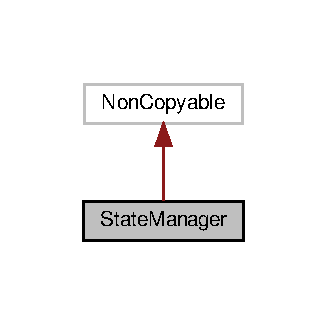
\includegraphics[width=157pt]{classStateManager__inherit__graph}
\end{center}
\end{figure}


Collaboration diagram for State\+Manager\+:
\nopagebreak
\begin{figure}[H]
\begin{center}
\leavevmode
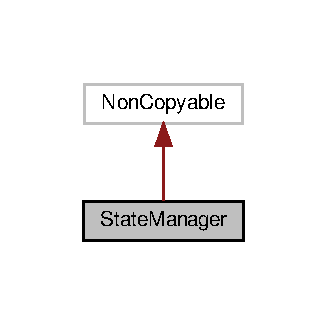
\includegraphics[width=157pt]{classStateManager__coll__graph}
\end{center}
\end{figure}
\subsection*{Public Types}
\begin{DoxyCompactItemize}
\item 
\mbox{\Hypertarget{classStateManager_a9f2dbb42af0109d58245e9d361df7a7b}\label{classStateManager_a9f2dbb42af0109d58245e9d361df7a7b}} 
enum \hyperlink{classStateManager_a9f2dbb42af0109d58245e9d361df7a7b}{Action} \{ {\bfseries Push}, 
{\bfseries Pop}, 
{\bfseries Clear}
 \}\begin{DoxyCompactList}\small\item\em three actions possibles for our management \end{DoxyCompactList}
\end{DoxyCompactItemize}
\subsection*{Public Member Functions}
\begin{DoxyCompactItemize}
\item 
\hyperlink{classStateManager_a4fbfb54fde50aefb32f8fd1cfe234c76}{State\+Manager} (\hyperlink{structState_1_1Context}{State\+::\+Context} context)
\begin{DoxyCompactList}\small\item\em Construct a new \hyperlink{classState}{State} Manager object. \end{DoxyCompactList}\item 
{\footnotesize template$<$typename T $>$ }\\void \hyperlink{classStateManager_a82f1a73f868174c930eb3d254b4eb7bb}{register\+State} (States\+::\+ID state\+ID)
\begin{DoxyCompactList}\small\item\em Polymorphic function to take all contexts as possible to work with. \end{DoxyCompactList}\item 
void \hyperlink{classStateManager_a07b3a4d61e0f75fc6c8730f9f77449a4}{update} (sf\+::\+Time dt)
\begin{DoxyCompactList}\small\item\em Iterate from top to bottom, stop as soon as \hyperlink{classStateManager_a07b3a4d61e0f75fc6c8730f9f77449a4}{update()} returns false. \end{DoxyCompactList}\item 
\mbox{\Hypertarget{classStateManager_a22666f2f72320ea3be46e9253b7530e2}\label{classStateManager_a22666f2f72320ea3be46e9253b7530e2}} 
void \hyperlink{classStateManager_a22666f2f72320ea3be46e9253b7530e2}{draw} ()
\begin{DoxyCompactList}\small\item\em Draw all active states from bottom to top. \end{DoxyCompactList}\item 
void \hyperlink{classStateManager_abe6bc824c376c7c5ec22b18b10b3ad92}{handle\+Event} (const sf\+::\+Event \&event)
\begin{DoxyCompactList}\small\item\em Iterate from top to bottom, stop as soon as \hyperlink{classStateManager_abe6bc824c376c7c5ec22b18b10b3ad92}{handle\+Event()} returns false. \end{DoxyCompactList}\item 
void \hyperlink{classStateManager_a4f0c970f9f5cdee29b16b1bc50614180}{push\+State} (States\+::\+ID state\+ID)
\begin{DoxyCompactList}\small\item\em Performing the status change for selected views. \end{DoxyCompactList}\item 
\mbox{\Hypertarget{classStateManager_a1c5f8c0609e74fb2346b6b7f5930bb38}\label{classStateManager_a1c5f8c0609e74fb2346b6b7f5930bb38}} 
void \hyperlink{classStateManager_a1c5f8c0609e74fb2346b6b7f5930bb38}{pop\+State} ()
\begin{DoxyCompactList}\small\item\em Putting stored views on the waiting list to active. \end{DoxyCompactList}\item 
\mbox{\Hypertarget{classStateManager_a3b18f37d97a6d9428daa21318b7381b3}\label{classStateManager_a3b18f37d97a6d9428daa21318b7381b3}} 
void \hyperlink{classStateManager_a3b18f37d97a6d9428daa21318b7381b3}{clear\+States} ()
\begin{DoxyCompactList}\small\item\em clears all storage states \end{DoxyCompactList}\item 
bool \hyperlink{classStateManager_ad66deb9a952a99c7c9943ebdbb7263d0}{is\+Empty} () const
\begin{DoxyCompactList}\small\item\em Check if the battery is empty or not. \end{DoxyCompactList}\end{DoxyCompactItemize}


\subsection{Constructor \& Destructor Documentation}
\mbox{\Hypertarget{classStateManager_a4fbfb54fde50aefb32f8fd1cfe234c76}\label{classStateManager_a4fbfb54fde50aefb32f8fd1cfe234c76}} 
\index{State\+Manager@{State\+Manager}!State\+Manager@{State\+Manager}}
\index{State\+Manager@{State\+Manager}!State\+Manager@{State\+Manager}}
\subsubsection{\texorpdfstring{State\+Manager()}{StateManager()}}
{\footnotesize\ttfamily State\+Manager\+::\+State\+Manager (\begin{DoxyParamCaption}\item[{\hyperlink{structState_1_1Context}{State\+::\+Context}}]{context }\end{DoxyParamCaption})\hspace{0.3cm}{\ttfamily [explicit]}}



Construct a new \hyperlink{classState}{State} Manager object. 


\begin{DoxyParams}{Parameters}
{\em context} & \\
\hline
\end{DoxyParams}


\subsection{Member Function Documentation}
\mbox{\Hypertarget{classStateManager_abe6bc824c376c7c5ec22b18b10b3ad92}\label{classStateManager_abe6bc824c376c7c5ec22b18b10b3ad92}} 
\index{State\+Manager@{State\+Manager}!handle\+Event@{handle\+Event}}
\index{handle\+Event@{handle\+Event}!State\+Manager@{State\+Manager}}
\subsubsection{\texorpdfstring{handle\+Event()}{handleEvent()}}
{\footnotesize\ttfamily void State\+Manager\+::handle\+Event (\begin{DoxyParamCaption}\item[{const sf\+::\+Event \&}]{event }\end{DoxyParamCaption})}



Iterate from top to bottom, stop as soon as \hyperlink{classStateManager_abe6bc824c376c7c5ec22b18b10b3ad92}{handle\+Event()} returns false. 


\begin{DoxyParams}{Parameters}
{\em event} & \\
\hline
\end{DoxyParams}
\mbox{\Hypertarget{classStateManager_ad66deb9a952a99c7c9943ebdbb7263d0}\label{classStateManager_ad66deb9a952a99c7c9943ebdbb7263d0}} 
\index{State\+Manager@{State\+Manager}!is\+Empty@{is\+Empty}}
\index{is\+Empty@{is\+Empty}!State\+Manager@{State\+Manager}}
\subsubsection{\texorpdfstring{is\+Empty()}{isEmpty()}}
{\footnotesize\ttfamily bool State\+Manager\+::is\+Empty (\begin{DoxyParamCaption}{ }\end{DoxyParamCaption}) const}



Check if the battery is empty or not. 

\begin{DoxyReturn}{Returns}
true 

false 
\end{DoxyReturn}
\mbox{\Hypertarget{classStateManager_a4f0c970f9f5cdee29b16b1bc50614180}\label{classStateManager_a4f0c970f9f5cdee29b16b1bc50614180}} 
\index{State\+Manager@{State\+Manager}!push\+State@{push\+State}}
\index{push\+State@{push\+State}!State\+Manager@{State\+Manager}}
\subsubsection{\texorpdfstring{push\+State()}{pushState()}}
{\footnotesize\ttfamily void State\+Manager\+::push\+State (\begin{DoxyParamCaption}\item[{States\+::\+ID}]{state\+ID }\end{DoxyParamCaption})}



Performing the status change for selected views. 


\begin{DoxyParams}{Parameters}
{\em state\+ID} & \\
\hline
\end{DoxyParams}
\mbox{\Hypertarget{classStateManager_a82f1a73f868174c930eb3d254b4eb7bb}\label{classStateManager_a82f1a73f868174c930eb3d254b4eb7bb}} 
\index{State\+Manager@{State\+Manager}!register\+State@{register\+State}}
\index{register\+State@{register\+State}!State\+Manager@{State\+Manager}}
\subsubsection{\texorpdfstring{register\+State()}{registerState()}}
{\footnotesize\ttfamily template$<$typename T $>$ \\
void State\+Manager\+::register\+State (\begin{DoxyParamCaption}\item[{States\+::\+ID}]{state\+ID }\end{DoxyParamCaption})}



Polymorphic function to take all contexts as possible to work with. 


\begin{DoxyParams}{Parameters}
{\em state\+ID} & \\
\hline
\end{DoxyParams}
\mbox{\Hypertarget{classStateManager_a07b3a4d61e0f75fc6c8730f9f77449a4}\label{classStateManager_a07b3a4d61e0f75fc6c8730f9f77449a4}} 
\index{State\+Manager@{State\+Manager}!update@{update}}
\index{update@{update}!State\+Manager@{State\+Manager}}
\subsubsection{\texorpdfstring{update()}{update()}}
{\footnotesize\ttfamily void State\+Manager\+::update (\begin{DoxyParamCaption}\item[{sf\+::\+Time}]{dt }\end{DoxyParamCaption})}



Iterate from top to bottom, stop as soon as \hyperlink{classStateManager_a07b3a4d61e0f75fc6c8730f9f77449a4}{update()} returns false. 


\begin{DoxyParams}{Parameters}
{\em dt} & \\
\hline
\end{DoxyParams}


The documentation for this class was generated from the following files\+:\begin{DoxyCompactItemize}
\item 
sources/utils/\+States/State\+Manager.\+hpp\item 
sources/utils/\+States/State\+Manager.\+cpp\end{DoxyCompactItemize}

\hypertarget{classTetromino}{}\section{Tetromino Class Reference}
\label{classTetromino}\index{Tetromino@{Tetromino}}
\subsection*{Public Types}
\begin{DoxyCompactItemize}
\item 
\mbox{\Hypertarget{classTetromino_a46651f8ddce680db2062abb69c213206}\label{classTetromino_a46651f8ddce680db2062abb69c213206}} 
typedef std\+::function$<$ void(Collision\+Direction cd)$>$ {\bfseries Callback}
\end{DoxyCompactItemize}
\subsection*{Public Member Functions}
\begin{DoxyCompactItemize}
\item 
int \hyperlink{classTetromino_aa77965d8aa40ea448b5e8c5e288910d0}{lowest\+Position} (bool axisY=true)
\begin{DoxyCompactList}\small\item\em Look for the smallest position between the X and Y values of the part in question. \end{DoxyCompactList}\item 
const std\+::vector$<$ sf\+::\+Vector2i $>$ \hyperlink{classTetromino_abbad824f47a492bdc96810908903c7ac}{get\+Stucture} ()
\begin{DoxyCompactList}\small\item\em Get the Stucture object current. \end{DoxyCompactList}\item 
\mbox{\Hypertarget{classTetromino_a16b078d3e8a3b75cf0e22aa64c46af5e}\label{classTetromino_a16b078d3e8a3b75cf0e22aa64c46af5e}} 
{\bfseries Tetromino} (int m\+BorderX, int m\+BorderY, Available\+Colors m\+Color)
\item 
\mbox{\Hypertarget{classTetromino_aeca0a1fc3b172f3545f8775e235d2d14}\label{classTetromino_aeca0a1fc3b172f3545f8775e235d2d14}} 
{\bfseries Tetromino} (int m\+BorderX, int m\+BorderY)
\item 
\mbox{\Hypertarget{classTetromino_a24fb8d502facca047e5e192cbc68a5ee}\label{classTetromino_a24fb8d502facca047e5e192cbc68a5ee}} 
{\bfseries Tetromino} (Available\+Colors m\+Color=Available\+Colors\+::\+T\+R\+A\+N\+S\+P\+A\+R\+E\+NT)
\item 
\mbox{\Hypertarget{classTetromino_ac87bbdae1c3c8349081f41327c0b4afb}\label{classTetromino_ac87bbdae1c3c8349081f41327c0b4afb}} 
{\bfseries Tetromino} (const \hyperlink{classTetromino}{Tetromino} \&t)
\item 
\hyperlink{classTetromino_ab2a8b2460d6acaf098cdc257630cd182}{Tetromino} (int m\+BorderX, int m\+BorderY, int offsetX, int offsetY, std\+::vector$<$ sf\+::\+Vector2i $>$ figure\+Structure, Available\+Colors m\+Color)
\item 
virtual void \hyperlink{classTetromino_ac1de8d2bbc2e46ee5d5586f25dcd4692}{rotate} (Direction d=Direction\+::\+C\+L\+O\+C\+K\+W\+I\+SE)
\begin{DoxyCompactList}\small\item\em uses the rotation function (x,y) = (y, -\/x) \end{DoxyCompactList}\item 
\mbox{\Hypertarget{classTetromino_a79f30c3dd8ea432e0bc5d7d2108e5a17}\label{classTetromino_a79f30c3dd8ea432e0bc5d7d2108e5a17}} 
void {\bfseries print} ()
\item 
\mbox{\Hypertarget{classTetromino_a612c515834ce52a37afe7ae39efcbd57}\label{classTetromino_a612c515834ce52a37afe7ae39efcbd57}} 
bool {\bfseries offset\+Axis} (bool axixY=true)
\item 
\mbox{\Hypertarget{classTetromino_a15a56c14bed5825cbb0da098bdba6ca2}\label{classTetromino_a15a56c14bed5825cbb0da098bdba6ca2}} 
void {\bfseries set\+Pos} (std\+::vector$<$ sf\+::\+Vector2i $>$ pos)
\item 
Available\+Colors \hyperlink{classTetromino_ad5594cc33ab35ec97b8eb3593e74b787}{get\+Color} ()
\begin{DoxyCompactList}\small\item\em Get the Color object. \end{DoxyCompactList}\item 
std\+::vector$<$ sf\+::\+Vector2i $>$ \hyperlink{classTetromino_a8c9202a6d41354fd5555cca89cec0703}{get\+Pos} ()
\begin{DoxyCompactList}\small\item\em Get the Pos of tetromino in table. \end{DoxyCompactList}\item 
void \hyperlink{classTetromino_a3ac5e896c58ed8490beac9ee833431e6}{set\+Collision\+Event} (Callback callback)
\begin{DoxyCompactList}\small\item\em Set the Collision Event to treat him and call the collision function. \end{DoxyCompactList}\item 
\hyperlink{classTetromino}{Tetromino} \& \hyperlink{classTetromino_ab4dd61078d1383df779f5f615d352a17}{operator++} (int)
\begin{DoxyCompactList}\small\item\em vertical movement of the tetromino \end{DoxyCompactList}\item 
\hyperlink{classTetromino}{Tetromino} \& \hyperlink{classTetromino_a3921b7fc54aca4d294b74b487d8c4183}{operator-\/-\/} (int)
\begin{DoxyCompactList}\small\item\em vertical movement of the tetromino \end{DoxyCompactList}\item 
bool \hyperlink{classTetromino_aea3c0024088f53627d766fba6a3fb4e4}{operator==} (\hyperlink{classMatrix}{Matrix} \&m)
\begin{DoxyCompactList}\small\item\em Insert value in the matrix directly just checking whether or not the space is available. \end{DoxyCompactList}\item 
bool \hyperlink{classTetromino_a1fb3c6bd848e94e099f74b7267b09bb2}{operator==} (\hyperlink{classTetromino}{Tetromino} \&t)
\begin{DoxyCompactList}\small\item\em Comparation between tetrominos. \end{DoxyCompactList}\item 
\mbox{\Hypertarget{classTetromino_a1b3d40f3fbe6707ade8c4ceabe0b470f}\label{classTetromino_a1b3d40f3fbe6707ade8c4ceabe0b470f}} 
void {\bfseries disable\+Event} ()
\item 
\mbox{\Hypertarget{classTetromino_a7a8183d917efd18738fc83ba86cfb010}\label{classTetromino_a7a8183d917efd18738fc83ba86cfb010}} 
void {\bfseries enable\+Event} ()
\item 
std\+::vector$<$ sf\+::\+Vector2i $>$ \hyperlink{classTetromino_ae067d0f05219f03a6b7f8e15e3cc67d0}{rotate\+Figure\+Structure} (Direction d=Direction\+::\+C\+L\+O\+C\+K\+W\+I\+SE)
\begin{DoxyCompactList}\small\item\em If it is possible to rotate the part according to the checking function, it is responsible for actually rotating the piece in real positions and fix it. \end{DoxyCompactList}\item 
sf\+::\+Vector2i \hyperlink{classTetromino_a6bcb8f93c3259bfba0bfa380c900af8a}{get\+Axis\+Coordinates} ()
\begin{DoxyCompactList}\small\item\em Get the Axis Coordinates object. \end{DoxyCompactList}\item 
int \hyperlink{classTetromino_aceb82d83a9a0c1d6825855e46c386b20}{get\+BorderX} ()
\begin{DoxyCompactList}\small\item\em Get the Border X object. \end{DoxyCompactList}\item 
int \hyperlink{classTetromino_a9ab14cf7ce0a87d9102c6b04f6f2f995}{get\+BorderY} ()
\begin{DoxyCompactList}\small\item\em Get the Border Y object. \end{DoxyCompactList}\item 
\hyperlink{classTetromino}{Tetromino} \hyperlink{classTetromino_aaf9f42f0c7432becc4e5f8fe47575f1b}{clone\+And\+Rotate} (Direction d=Direction\+::\+C\+L\+O\+C\+K\+W\+I\+SE)
\begin{DoxyCompactList}\small\item\em Clone the part before rotating it, if the clone can be fitted into the matrix, it will assume the original position, thus making the rotation movement. \end{DoxyCompactList}\item 
\mbox{\Hypertarget{classTetromino_a28d82770c123148f13468456a4508353}\label{classTetromino_a28d82770c123148f13468456a4508353}} 
void \hyperlink{classTetromino_a28d82770c123148f13468456a4508353}{correct\+Border} ()
\begin{DoxyCompactList}\small\item\em Check if there is a conflict between the edges of the matrix, and if there is, make the right correction so as not to blast the boundaries. \end{DoxyCompactList}\end{DoxyCompactItemize}
\subsection*{Friends}
\begin{DoxyCompactItemize}
\item 
\hyperlink{classTetromino}{Tetromino} \& \hyperlink{classTetromino_a6df1d7b28f8b0b41027018105153cc42}{operator+} (const \hyperlink{classTetromino}{Tetromino} \&t1, const int offsetX)
\begin{DoxyCompactList}\small\item\em Make the movement in x, making the horizontal movement of the piece in which we move in the positive direction. \end{DoxyCompactList}\item 
\hyperlink{classTetromino}{Tetromino} \& \hyperlink{classTetromino_ac382287ca988f74d5a2e517224a1dfd4}{operator-\/} (const \hyperlink{classTetromino}{Tetromino} \&t1, const int offsetX)
\begin{DoxyCompactList}\small\item\em Make the movement in x, making the horizontal movement of the piece in which we move in the negative direction. \end{DoxyCompactList}\end{DoxyCompactItemize}


\subsection{Constructor \& Destructor Documentation}
\mbox{\Hypertarget{classTetromino_ab2a8b2460d6acaf098cdc257630cd182}\label{classTetromino_ab2a8b2460d6acaf098cdc257630cd182}} 
\index{Tetromino@{Tetromino}!Tetromino@{Tetromino}}
\index{Tetromino@{Tetromino}!Tetromino@{Tetromino}}
\subsubsection{\texorpdfstring{Tetromino()}{Tetromino()}}
{\footnotesize\ttfamily Tetromino\+::\+Tetromino (\begin{DoxyParamCaption}\item[{int}]{m\+BorderX,  }\item[{int}]{m\+BorderY,  }\item[{int}]{offsetX,  }\item[{int}]{offsetY,  }\item[{std\+::vector$<$ sf\+::\+Vector2i $>$}]{figure\+Structure,  }\item[{Available\+Colors}]{m\+Color }\end{DoxyParamCaption})}

T\+O\+DO\+: Validate the distances between the size

add cassert

\subsection{Member Function Documentation}
\mbox{\Hypertarget{classTetromino_aaf9f42f0c7432becc4e5f8fe47575f1b}\label{classTetromino_aaf9f42f0c7432becc4e5f8fe47575f1b}} 
\index{Tetromino@{Tetromino}!clone\+And\+Rotate@{clone\+And\+Rotate}}
\index{clone\+And\+Rotate@{clone\+And\+Rotate}!Tetromino@{Tetromino}}
\subsubsection{\texorpdfstring{clone\+And\+Rotate()}{cloneAndRotate()}}
{\footnotesize\ttfamily \hyperlink{classTetromino}{Tetromino} Tetromino\+::clone\+And\+Rotate (\begin{DoxyParamCaption}\item[{Direction}]{d = {\ttfamily Direction\+:\+:CLOCKWISE} }\end{DoxyParamCaption})}



Clone the part before rotating it, if the clone can be fitted into the matrix, it will assume the original position, thus making the rotation movement. 


\begin{DoxyParams}{Parameters}
{\em d} & \\
\hline
\end{DoxyParams}
\begin{DoxyReturn}{Returns}
\hyperlink{classTetromino}{Tetromino} 
\end{DoxyReturn}
\mbox{\Hypertarget{classTetromino_a6bcb8f93c3259bfba0bfa380c900af8a}\label{classTetromino_a6bcb8f93c3259bfba0bfa380c900af8a}} 
\index{Tetromino@{Tetromino}!get\+Axis\+Coordinates@{get\+Axis\+Coordinates}}
\index{get\+Axis\+Coordinates@{get\+Axis\+Coordinates}!Tetromino@{Tetromino}}
\subsubsection{\texorpdfstring{get\+Axis\+Coordinates()}{getAxisCoordinates()}}
{\footnotesize\ttfamily sf\+::\+Vector2i Tetromino\+::get\+Axis\+Coordinates (\begin{DoxyParamCaption}{ }\end{DoxyParamCaption})}



Get the Axis Coordinates object. 

\begin{DoxyReturn}{Returns}
sf\+::\+Vector2i in (x,y) 
\end{DoxyReturn}
\mbox{\Hypertarget{classTetromino_aceb82d83a9a0c1d6825855e46c386b20}\label{classTetromino_aceb82d83a9a0c1d6825855e46c386b20}} 
\index{Tetromino@{Tetromino}!get\+BorderX@{get\+BorderX}}
\index{get\+BorderX@{get\+BorderX}!Tetromino@{Tetromino}}
\subsubsection{\texorpdfstring{get\+Border\+X()}{getBorderX()}}
{\footnotesize\ttfamily int Tetromino\+::get\+BorderX (\begin{DoxyParamCaption}{ }\end{DoxyParamCaption})}



Get the Border X object. 

\begin{DoxyReturn}{Returns}
int 
\end{DoxyReturn}
\mbox{\Hypertarget{classTetromino_a9ab14cf7ce0a87d9102c6b04f6f2f995}\label{classTetromino_a9ab14cf7ce0a87d9102c6b04f6f2f995}} 
\index{Tetromino@{Tetromino}!get\+BorderY@{get\+BorderY}}
\index{get\+BorderY@{get\+BorderY}!Tetromino@{Tetromino}}
\subsubsection{\texorpdfstring{get\+Border\+Y()}{getBorderY()}}
{\footnotesize\ttfamily int Tetromino\+::get\+BorderY (\begin{DoxyParamCaption}{ }\end{DoxyParamCaption})}



Get the Border Y object. 

\begin{DoxyReturn}{Returns}
int 
\end{DoxyReturn}
\mbox{\Hypertarget{classTetromino_ad5594cc33ab35ec97b8eb3593e74b787}\label{classTetromino_ad5594cc33ab35ec97b8eb3593e74b787}} 
\index{Tetromino@{Tetromino}!get\+Color@{get\+Color}}
\index{get\+Color@{get\+Color}!Tetromino@{Tetromino}}
\subsubsection{\texorpdfstring{get\+Color()}{getColor()}}
{\footnotesize\ttfamily Available\+Colors Tetromino\+::get\+Color (\begin{DoxyParamCaption}{ }\end{DoxyParamCaption})}



Get the Color object. 

\begin{DoxyReturn}{Returns}
the color of piece 
\end{DoxyReturn}
\mbox{\Hypertarget{classTetromino_a8c9202a6d41354fd5555cca89cec0703}\label{classTetromino_a8c9202a6d41354fd5555cca89cec0703}} 
\index{Tetromino@{Tetromino}!get\+Pos@{get\+Pos}}
\index{get\+Pos@{get\+Pos}!Tetromino@{Tetromino}}
\subsubsection{\texorpdfstring{get\+Pos()}{getPos()}}
{\footnotesize\ttfamily std\+::vector$<$ sf\+::\+Vector2i $>$ Tetromino\+::get\+Pos (\begin{DoxyParamCaption}{ }\end{DoxyParamCaption})}



Get the Pos of tetromino in table. 

\begin{DoxyReturn}{Returns}
(x;y) 
\end{DoxyReturn}
\mbox{\Hypertarget{classTetromino_abbad824f47a492bdc96810908903c7ac}\label{classTetromino_abbad824f47a492bdc96810908903c7ac}} 
\index{Tetromino@{Tetromino}!get\+Stucture@{get\+Stucture}}
\index{get\+Stucture@{get\+Stucture}!Tetromino@{Tetromino}}
\subsubsection{\texorpdfstring{get\+Stucture()}{getStucture()}}
{\footnotesize\ttfamily const std\+::vector$<$ sf\+::\+Vector2i $>$ Tetromino\+::get\+Stucture (\begin{DoxyParamCaption}{ }\end{DoxyParamCaption})}



Get the Stucture object current. 

\begin{DoxyReturn}{Returns}
const std\+::vector$<$sf\+::\+Vector2i$>$ with positions in content 
\end{DoxyReturn}
\mbox{\Hypertarget{classTetromino_aa77965d8aa40ea448b5e8c5e288910d0}\label{classTetromino_aa77965d8aa40ea448b5e8c5e288910d0}} 
\index{Tetromino@{Tetromino}!lowest\+Position@{lowest\+Position}}
\index{lowest\+Position@{lowest\+Position}!Tetromino@{Tetromino}}
\subsubsection{\texorpdfstring{lowest\+Position()}{lowestPosition()}}
{\footnotesize\ttfamily int Tetromino\+::lowest\+Position (\begin{DoxyParamCaption}\item[{bool}]{axisY = {\ttfamily true} }\end{DoxyParamCaption})}



Look for the smallest position between the X and Y values of the part in question. 


\begin{DoxyParams}{Parameters}
{\em axisY} & \\
\hline
\end{DoxyParams}
\begin{DoxyReturn}{Returns}
int value of lowest position between x and y 
\end{DoxyReturn}
\mbox{\Hypertarget{classTetromino_ab4dd61078d1383df779f5f615d352a17}\label{classTetromino_ab4dd61078d1383df779f5f615d352a17}} 
\index{Tetromino@{Tetromino}!operator++@{operator++}}
\index{operator++@{operator++}!Tetromino@{Tetromino}}
\subsubsection{\texorpdfstring{operator++()}{operator++()}}
{\footnotesize\ttfamily \hyperlink{classTetromino}{Tetromino} \& Tetromino\+::operator++ (\begin{DoxyParamCaption}\item[{int}]{ }\end{DoxyParamCaption})}



vertical movement of the tetromino 

\begin{DoxyReturn}{Returns}
\hyperlink{classTetromino}{Tetromino}\& 
\end{DoxyReturn}
\mbox{\Hypertarget{classTetromino_a3921b7fc54aca4d294b74b487d8c4183}\label{classTetromino_a3921b7fc54aca4d294b74b487d8c4183}} 
\index{Tetromino@{Tetromino}!operator-\/-\/@{operator-\/-\/}}
\index{operator-\/-\/@{operator-\/-\/}!Tetromino@{Tetromino}}
\subsubsection{\texorpdfstring{operator-\/-\/()}{operator--()}}
{\footnotesize\ttfamily \hyperlink{classTetromino}{Tetromino} \& Tetromino\+::operator-\/-\/ (\begin{DoxyParamCaption}\item[{int}]{ }\end{DoxyParamCaption})}



vertical movement of the tetromino 

\begin{DoxyReturn}{Returns}
\hyperlink{classTetromino}{Tetromino}\& 
\end{DoxyReturn}
\mbox{\Hypertarget{classTetromino_aea3c0024088f53627d766fba6a3fb4e4}\label{classTetromino_aea3c0024088f53627d766fba6a3fb4e4}} 
\index{Tetromino@{Tetromino}!operator==@{operator==}}
\index{operator==@{operator==}!Tetromino@{Tetromino}}
\subsubsection{\texorpdfstring{operator==()}{operator==()}\hspace{0.1cm}{\footnotesize\ttfamily [1/2]}}
{\footnotesize\ttfamily bool Tetromino\+::operator== (\begin{DoxyParamCaption}\item[{\hyperlink{classMatrix}{Matrix} \&}]{m }\end{DoxyParamCaption})}



Insert value in the matrix directly just checking whether or not the space is available. 


\begin{DoxyParams}{Parameters}
{\em m} & \\
\hline
\end{DoxyParams}
\begin{DoxyReturn}{Returns}
true 

false 
\end{DoxyReturn}
\mbox{\Hypertarget{classTetromino_a1fb3c6bd848e94e099f74b7267b09bb2}\label{classTetromino_a1fb3c6bd848e94e099f74b7267b09bb2}} 
\index{Tetromino@{Tetromino}!operator==@{operator==}}
\index{operator==@{operator==}!Tetromino@{Tetromino}}
\subsubsection{\texorpdfstring{operator==()}{operator==()}\hspace{0.1cm}{\footnotesize\ttfamily [2/2]}}
{\footnotesize\ttfamily bool Tetromino\+::operator== (\begin{DoxyParamCaption}\item[{\hyperlink{classTetromino}{Tetromino} \&}]{t }\end{DoxyParamCaption})}



Comparation between tetrominos. 


\begin{DoxyParams}{Parameters}
{\em t} & \\
\hline
\end{DoxyParams}
\begin{DoxyReturn}{Returns}
true 

false 
\end{DoxyReturn}
\mbox{\Hypertarget{classTetromino_ac1de8d2bbc2e46ee5d5586f25dcd4692}\label{classTetromino_ac1de8d2bbc2e46ee5d5586f25dcd4692}} 
\index{Tetromino@{Tetromino}!rotate@{rotate}}
\index{rotate@{rotate}!Tetromino@{Tetromino}}
\subsubsection{\texorpdfstring{rotate()}{rotate()}}
{\footnotesize\ttfamily void Tetromino\+::rotate (\begin{DoxyParamCaption}\item[{Direction}]{d = {\ttfamily Direction\+:\+:CLOCKWISE} }\end{DoxyParamCaption})\hspace{0.3cm}{\ttfamily [virtual]}}



uses the rotation function (x,y) = (y, -\/x) 


\begin{DoxyParams}{Parameters}
{\em d} & orientation\+: Clokwise or anti-\/clockwise \\
\hline
\end{DoxyParams}
\mbox{\Hypertarget{classTetromino_ae067d0f05219f03a6b7f8e15e3cc67d0}\label{classTetromino_ae067d0f05219f03a6b7f8e15e3cc67d0}} 
\index{Tetromino@{Tetromino}!rotate\+Figure\+Structure@{rotate\+Figure\+Structure}}
\index{rotate\+Figure\+Structure@{rotate\+Figure\+Structure}!Tetromino@{Tetromino}}
\subsubsection{\texorpdfstring{rotate\+Figure\+Structure()}{rotateFigureStructure()}}
{\footnotesize\ttfamily std\+::vector$<$ sf\+::\+Vector2i $>$ Tetromino\+::rotate\+Figure\+Structure (\begin{DoxyParamCaption}\item[{Direction}]{d = {\ttfamily Direction\+:\+:CLOCKWISE} }\end{DoxyParamCaption})}



If it is possible to rotate the part according to the checking function, it is responsible for actually rotating the piece in real positions and fix it. 


\begin{DoxyParams}{Parameters}
{\em d} & \\
\hline
\end{DoxyParams}
\begin{DoxyReturn}{Returns}
std\+::vector$<$sf\+::\+Vector2i$>$ 
\end{DoxyReturn}
\mbox{\Hypertarget{classTetromino_a3ac5e896c58ed8490beac9ee833431e6}\label{classTetromino_a3ac5e896c58ed8490beac9ee833431e6}} 
\index{Tetromino@{Tetromino}!set\+Collision\+Event@{set\+Collision\+Event}}
\index{set\+Collision\+Event@{set\+Collision\+Event}!Tetromino@{Tetromino}}
\subsubsection{\texorpdfstring{set\+Collision\+Event()}{setCollisionEvent()}}
{\footnotesize\ttfamily void Tetromino\+::set\+Collision\+Event (\begin{DoxyParamCaption}\item[{Callback}]{callback }\end{DoxyParamCaption})}



Set the Collision Event to treat him and call the collision function. 


\begin{DoxyParams}{Parameters}
{\em callback} & \\
\hline
\end{DoxyParams}


\subsection{Friends And Related Function Documentation}
\mbox{\Hypertarget{classTetromino_a6df1d7b28f8b0b41027018105153cc42}\label{classTetromino_a6df1d7b28f8b0b41027018105153cc42}} 
\index{Tetromino@{Tetromino}!operator+@{operator+}}
\index{operator+@{operator+}!Tetromino@{Tetromino}}
\subsubsection{\texorpdfstring{operator+}{operator+}}
{\footnotesize\ttfamily \hyperlink{classTetromino}{Tetromino}\& operator+ (\begin{DoxyParamCaption}\item[{const \hyperlink{classTetromino}{Tetromino} \&}]{t1,  }\item[{const int}]{offsetX }\end{DoxyParamCaption})\hspace{0.3cm}{\ttfamily [friend]}}



Make the movement in x, making the horizontal movement of the piece in which we move in the positive direction. 


\begin{DoxyParams}{Parameters}
{\em t1} & \\
\hline
{\em offsetX} & \\
\hline
\end{DoxyParams}
\begin{DoxyReturn}{Returns}
\hyperlink{classTetromino}{Tetromino}\& 
\end{DoxyReturn}
\mbox{\Hypertarget{classTetromino_ac382287ca988f74d5a2e517224a1dfd4}\label{classTetromino_ac382287ca988f74d5a2e517224a1dfd4}} 
\index{Tetromino@{Tetromino}!operator-\/@{operator-\/}}
\index{operator-\/@{operator-\/}!Tetromino@{Tetromino}}
\subsubsection{\texorpdfstring{operator-\/}{operator-}}
{\footnotesize\ttfamily \hyperlink{classTetromino}{Tetromino}\& operator-\/ (\begin{DoxyParamCaption}\item[{const \hyperlink{classTetromino}{Tetromino} \&}]{t1,  }\item[{const int}]{offsetX }\end{DoxyParamCaption})\hspace{0.3cm}{\ttfamily [friend]}}



Make the movement in x, making the horizontal movement of the piece in which we move in the negative direction. 


\begin{DoxyParams}{Parameters}
{\em t1} & \\
\hline
{\em offsetX} & \\
\hline
\end{DoxyParams}
\begin{DoxyReturn}{Returns}
\hyperlink{classTetromino}{Tetromino}\& 
\end{DoxyReturn}


The documentation for this class was generated from the following files\+:\begin{DoxyCompactItemize}
\item 
sources/game/Tetromino.\+hpp\item 
sources/game/Tetromino.\+cpp\end{DoxyCompactItemize}

\hypertarget{classTitleScene}{}\section{Title\+Scene Class Reference}
\label{classTitleScene}\index{Title\+Scene@{Title\+Scene}}


class responsible for taking care of the initial screen of the game  




{\ttfamily \#include $<$Title\+Scene.\+hpp$>$}



Inheritance diagram for Title\+Scene\+:
\nopagebreak
\begin{figure}[H]
\begin{center}
\leavevmode
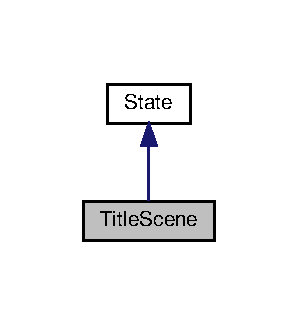
\includegraphics[width=143pt]{classTitleScene__inherit__graph}
\end{center}
\end{figure}


Collaboration diagram for Title\+Scene\+:
\nopagebreak
\begin{figure}[H]
\begin{center}
\leavevmode
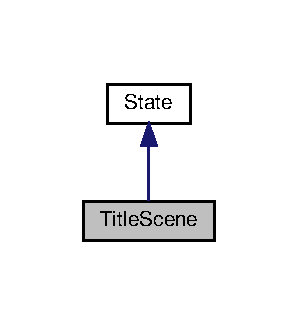
\includegraphics[width=143pt]{classTitleScene__coll__graph}
\end{center}
\end{figure}
\subsection*{Public Member Functions}
\begin{DoxyCompactItemize}
\item 
\hyperlink{classTitleScene_a2542c8d7f2bcd75f69d79ec96cf75859}{Title\+Scene} (\hyperlink{classStateManager}{State\+Manager} \&stack, \hyperlink{structState_1_1Context}{Context} context)
\begin{DoxyCompactList}\small\item\em Construct a new Title Scene object, standard builder. \end{DoxyCompactList}\item 
\mbox{\Hypertarget{classTitleScene_af9939b69acd5a381b53678f022928110}\label{classTitleScene_af9939b69acd5a381b53678f022928110}} 
virtual void \hyperlink{classTitleScene_af9939b69acd5a381b53678f022928110}{draw} ()
\begin{DoxyCompactList}\small\item\em overwriting the function drawing by adding new elements responsible for sampling new elements added to this view \end{DoxyCompactList}\item 
virtual bool \hyperlink{classTitleScene_a7da09182894a7a48a12ed0e170e5b5f3}{update} (sf\+::\+Time dt)
\begin{DoxyCompactList}\small\item\em overwriting the function update by adding new elements responsible for sampling new elements added to this view \end{DoxyCompactList}\item 
virtual bool \hyperlink{classTitleScene_ae965e4a6c1435246fcbdd487bbc58468}{handle\+Event} (const sf\+::\+Event \&event)
\begin{DoxyCompactList}\small\item\em Adds new features to the function responsible for handling the events, adding a specific function for each key depending on the view. \end{DoxyCompactList}\end{DoxyCompactItemize}
\subsection*{Additional Inherited Members}


\subsection{Detailed Description}
class responsible for taking care of the initial screen of the game 

\subsection{Constructor \& Destructor Documentation}
\mbox{\Hypertarget{classTitleScene_a2542c8d7f2bcd75f69d79ec96cf75859}\label{classTitleScene_a2542c8d7f2bcd75f69d79ec96cf75859}} 
\index{Title\+Scene@{Title\+Scene}!Title\+Scene@{Title\+Scene}}
\index{Title\+Scene@{Title\+Scene}!Title\+Scene@{Title\+Scene}}
\subsubsection{\texorpdfstring{Title\+Scene()}{TitleScene()}}
{\footnotesize\ttfamily Title\+Scene\+::\+Title\+Scene (\begin{DoxyParamCaption}\item[{\hyperlink{classStateManager}{State\+Manager} \&}]{stack,  }\item[{\hyperlink{structState_1_1Context}{Context}}]{context }\end{DoxyParamCaption})}



Construct a new Title Scene object, standard builder. 


\begin{DoxyParams}{Parameters}
{\em stack} & stack responsible for managing the views \\
\hline
{\em context} & relates all current context \\
\hline
\end{DoxyParams}


\subsection{Member Function Documentation}
\mbox{\Hypertarget{classTitleScene_ae965e4a6c1435246fcbdd487bbc58468}\label{classTitleScene_ae965e4a6c1435246fcbdd487bbc58468}} 
\index{Title\+Scene@{Title\+Scene}!handle\+Event@{handle\+Event}}
\index{handle\+Event@{handle\+Event}!Title\+Scene@{Title\+Scene}}
\subsubsection{\texorpdfstring{handle\+Event()}{handleEvent()}}
{\footnotesize\ttfamily bool Title\+Scene\+::handle\+Event (\begin{DoxyParamCaption}\item[{const sf\+::\+Event \&}]{event }\end{DoxyParamCaption})\hspace{0.3cm}{\ttfamily [virtual]}}



Adds new features to the function responsible for handling the events, adding a specific function for each key depending on the view. 


\begin{DoxyParams}{Parameters}
{\em event} & getted action \\
\hline
\end{DoxyParams}
\begin{DoxyReturn}{Returns}
true 

false if have a problem 
\end{DoxyReturn}


Implements \hyperlink{classState_a19965f83460b248c42952aac8d001206}{State}.

\mbox{\Hypertarget{classTitleScene_a7da09182894a7a48a12ed0e170e5b5f3}\label{classTitleScene_a7da09182894a7a48a12ed0e170e5b5f3}} 
\index{Title\+Scene@{Title\+Scene}!update@{update}}
\index{update@{update}!Title\+Scene@{Title\+Scene}}
\subsubsection{\texorpdfstring{update()}{update()}}
{\footnotesize\ttfamily bool Title\+Scene\+::update (\begin{DoxyParamCaption}\item[{sf\+::\+Time}]{dt }\end{DoxyParamCaption})\hspace{0.3cm}{\ttfamily [virtual]}}



overwriting the function update by adding new elements responsible for sampling new elements added to this view 


\begin{DoxyParams}{Parameters}
{\em dt} & Fraction of time \\
\hline
\end{DoxyParams}
\begin{DoxyReturn}{Returns}
true 

false if have a problem 
\end{DoxyReturn}


Implements \hyperlink{classState_acd5926bc7a373edff9e57f3ffe94ca13}{State}.



The documentation for this class was generated from the following files\+:\begin{DoxyCompactItemize}
\item 
sources/views/Title\+Scene.\+hpp\item 
sources/views/Title\+Scene.\+cpp\end{DoxyCompactItemize}

\hypertarget{classUtility}{}\section{Utility Class Reference}
\label{classUtility}\index{Utility@{Utility}}


Class that contains utilities to facilitate uses, such as relative positions, and take center screen.  




{\ttfamily \#include $<$Utility.\+hpp$>$}

\subsection*{Static Public Member Functions}
\begin{DoxyCompactItemize}
\item 
static void \hyperlink{classUtility_a740b125c33224b1845cc8cd34481344f}{center\+Origin} (sf\+::\+Sprite \&sprite)
\begin{DoxyCompactList}\small\item\em Places a sprite in the center of the screen being managed. \end{DoxyCompactList}\item 
static void \hyperlink{classUtility_afb1f918173dab3a113304952b7d5fb86}{center\+Origin} (sf\+::\+Shape \&sprite)
\begin{DoxyCompactList}\small\item\em Places a Shape in the center of the screen being managed. \end{DoxyCompactList}\item 
static void \hyperlink{classUtility_ac60c8088a90a2839e35d79d8ac8c8a50}{center\+Origin} (sf\+::\+Text \&text)
\begin{DoxyCompactList}\small\item\em Places in the center of the screen texts. \end{DoxyCompactList}\item 
static const sf\+::\+Vector2f \hyperlink{classUtility_adc3cdc839cb23f7fcbaee921bdeecbb2}{get\+Position\+Relative} (sf\+::\+Vector2u sv, unsigned int propX, unsigned int propY, int displacementX=1, int displacementY=1)
\begin{DoxyCompactList}\small\item\em Get the Position Relative object, cutting the screen into strips, as in a large mesh, and choosing to position the element between its x,y. \end{DoxyCompactList}\item 
static const sf\+::\+Vector2f \hyperlink{classUtility_a4eedd5b332f25c2fd8b8aaa21e104b71}{get\+Position\+Relative} (sf\+::\+Vector2f sv, unsigned int propX, unsigned int propY, int displacementX=1, int displacementY=1)
\begin{DoxyCompactList}\small\item\em Get the Position Relative object, cutting the screen into strips, as in a large mesh, and choosing to position the element between its x,y. \end{DoxyCompactList}\item 
static const sf\+::\+Int\+Rect \hyperlink{classUtility_a0fb51a6c84ab339bb52434a8b805fa20}{get\+Rect\+Window} (int displacementX=0, int displacementY=0)
\begin{DoxyCompactList}\small\item\em Get the Rect Window object. \end{DoxyCompactList}\end{DoxyCompactItemize}
\subsection*{Static Public Attributes}
\begin{DoxyCompactItemize}
\item 
\mbox{\Hypertarget{classUtility_a417cff4a0f693a4fd0e7bd93af05a351}\label{classUtility_a417cff4a0f693a4fd0e7bd93af05a351}} 
static const sf\+::\+Vector2f {\bfseries W\+I\+N\+D\+O\+W\+\_\+\+S\+I\+ZE} = sf\+::\+Vector2f(1024, 576)
\end{DoxyCompactItemize}


\subsection{Detailed Description}
Class that contains utilities to facilitate uses, such as relative positions, and take center screen. 

\subsection{Member Function Documentation}
\mbox{\Hypertarget{classUtility_a740b125c33224b1845cc8cd34481344f}\label{classUtility_a740b125c33224b1845cc8cd34481344f}} 
\index{Utility@{Utility}!center\+Origin@{center\+Origin}}
\index{center\+Origin@{center\+Origin}!Utility@{Utility}}
\subsubsection{\texorpdfstring{center\+Origin()}{centerOrigin()}\hspace{0.1cm}{\footnotesize\ttfamily [1/3]}}
{\footnotesize\ttfamily void Utility\+::center\+Origin (\begin{DoxyParamCaption}\item[{sf\+::\+Sprite \&}]{sprite }\end{DoxyParamCaption})\hspace{0.3cm}{\ttfamily [static]}}



Places a sprite in the center of the screen being managed. 


\begin{DoxyParams}{Parameters}
{\em sprite} & ex\+: background figures (sf\+::\+Sprite) \\
\hline
\end{DoxyParams}
\mbox{\Hypertarget{classUtility_afb1f918173dab3a113304952b7d5fb86}\label{classUtility_afb1f918173dab3a113304952b7d5fb86}} 
\index{Utility@{Utility}!center\+Origin@{center\+Origin}}
\index{center\+Origin@{center\+Origin}!Utility@{Utility}}
\subsubsection{\texorpdfstring{center\+Origin()}{centerOrigin()}\hspace{0.1cm}{\footnotesize\ttfamily [2/3]}}
{\footnotesize\ttfamily void Utility\+::center\+Origin (\begin{DoxyParamCaption}\item[{sf\+::\+Shape \&}]{sprite }\end{DoxyParamCaption})\hspace{0.3cm}{\ttfamily [static]}}



Places a Shape in the center of the screen being managed. 


\begin{DoxyParams}{Parameters}
{\em sprite} & forms generated by sf\+::\+Shape, etc. \\
\hline
\end{DoxyParams}
\mbox{\Hypertarget{classUtility_ac60c8088a90a2839e35d79d8ac8c8a50}\label{classUtility_ac60c8088a90a2839e35d79d8ac8c8a50}} 
\index{Utility@{Utility}!center\+Origin@{center\+Origin}}
\index{center\+Origin@{center\+Origin}!Utility@{Utility}}
\subsubsection{\texorpdfstring{center\+Origin()}{centerOrigin()}\hspace{0.1cm}{\footnotesize\ttfamily [3/3]}}
{\footnotesize\ttfamily void Utility\+::center\+Origin (\begin{DoxyParamCaption}\item[{sf\+::\+Text \&}]{text }\end{DoxyParamCaption})\hspace{0.3cm}{\ttfamily [static]}}



Places in the center of the screen texts. 


\begin{DoxyParams}{Parameters}
{\em text} & generate by sf\+::\+Text\\
\hline
\end{DoxyParams}
T\+O\+DO\+: Migrate everything to templates \mbox{\Hypertarget{classUtility_adc3cdc839cb23f7fcbaee921bdeecbb2}\label{classUtility_adc3cdc839cb23f7fcbaee921bdeecbb2}} 
\index{Utility@{Utility}!get\+Position\+Relative@{get\+Position\+Relative}}
\index{get\+Position\+Relative@{get\+Position\+Relative}!Utility@{Utility}}
\subsubsection{\texorpdfstring{get\+Position\+Relative()}{getPositionRelative()}\hspace{0.1cm}{\footnotesize\ttfamily [1/2]}}
{\footnotesize\ttfamily const sf\+::\+Vector2f Utility\+::get\+Position\+Relative (\begin{DoxyParamCaption}\item[{sf\+::\+Vector2u}]{sv,  }\item[{unsigned int}]{propX,  }\item[{unsigned int}]{propY,  }\item[{int}]{displacementX = {\ttfamily 1},  }\item[{int}]{displacementY = {\ttfamily 1} }\end{DoxyParamCaption})\hspace{0.3cm}{\ttfamily [static]}}



Get the Position Relative object, cutting the screen into strips, as in a large mesh, and choosing to position the element between its x,y. 


\begin{DoxyParams}{Parameters}
{\em sv} & Vector2u relative to screen size \\
\hline
{\em propX} & Cuts in x \\
\hline
{\em propY} & Cuts in y \\
\hline
{\em displacementX} & position x \\
\hline
{\em displacementY} & position y \\
\hline
\end{DoxyParams}
\begin{DoxyReturn}{Returns}
const sf\+::\+Vector2f with coordenates x,y 
\end{DoxyReturn}
\mbox{\Hypertarget{classUtility_a4eedd5b332f25c2fd8b8aaa21e104b71}\label{classUtility_a4eedd5b332f25c2fd8b8aaa21e104b71}} 
\index{Utility@{Utility}!get\+Position\+Relative@{get\+Position\+Relative}}
\index{get\+Position\+Relative@{get\+Position\+Relative}!Utility@{Utility}}
\subsubsection{\texorpdfstring{get\+Position\+Relative()}{getPositionRelative()}\hspace{0.1cm}{\footnotesize\ttfamily [2/2]}}
{\footnotesize\ttfamily const sf\+::\+Vector2f Utility\+::get\+Position\+Relative (\begin{DoxyParamCaption}\item[{sf\+::\+Vector2f}]{sv,  }\item[{unsigned int}]{propX,  }\item[{unsigned int}]{propY,  }\item[{int}]{displacementX = {\ttfamily 1},  }\item[{int}]{displacementY = {\ttfamily 1} }\end{DoxyParamCaption})\hspace{0.3cm}{\ttfamily [static]}}



Get the Position Relative object, cutting the screen into strips, as in a large mesh, and choosing to position the element between its x,y. 


\begin{DoxyParams}{Parameters}
{\em sv} & Vector2f relative to screen size \\
\hline
{\em propX} & Cuts in x \\
\hline
{\em propY} & Cuts in y \\
\hline
{\em displacementX} & position x \\
\hline
{\em displacementY} & position y \\
\hline
\end{DoxyParams}
\begin{DoxyReturn}{Returns}
const sf\+::\+Vector2f with coordenates x,y 
\end{DoxyReturn}
\mbox{\Hypertarget{classUtility_a0fb51a6c84ab339bb52434a8b805fa20}\label{classUtility_a0fb51a6c84ab339bb52434a8b805fa20}} 
\index{Utility@{Utility}!get\+Rect\+Window@{get\+Rect\+Window}}
\index{get\+Rect\+Window@{get\+Rect\+Window}!Utility@{Utility}}
\subsubsection{\texorpdfstring{get\+Rect\+Window()}{getRectWindow()}}
{\footnotesize\ttfamily const sf\+::\+Int\+Rect Utility\+::get\+Rect\+Window (\begin{DoxyParamCaption}\item[{int}]{displacementX = {\ttfamily 0},  }\item[{int}]{displacementY = {\ttfamily 0} }\end{DoxyParamCaption})\hspace{0.3cm}{\ttfamily [static]}}



Get the Rect Window object. 


\begin{DoxyParams}{Parameters}
{\em displacementX} & \\
\hline
{\em displacementY} & \\
\hline
\end{DoxyParams}
\begin{DoxyReturn}{Returns}
const sf\+::\+Int\+Rect 
\end{DoxyReturn}


The documentation for this class was generated from the following files\+:\begin{DoxyCompactItemize}
\item 
sources/utils/Utility.\+hpp\item 
sources/utils/Utility.\+cpp\end{DoxyCompactItemize}

\chapter{File Documentation}
\hypertarget{States_8hpp}{}\section{sources/utils/\+States.hpp File Reference}
\label{States_8hpp}\index{sources/utils/\+States.\+hpp@{sources/utils/\+States.\+hpp}}


Compilation of paths to add State-\/related libraries.  


{\ttfamily \#include \char`\"{}./\+States/\+State\+Identifiers.\+hpp\char`\"{}}\newline
{\ttfamily \#include \char`\"{}./\+States/\+State.\+hpp\char`\"{}}\newline
{\ttfamily \#include \char`\"{}./\+States/\+State\+Manager.\+hpp\char`\"{}}\newline
Include dependency graph for States.\+hpp\+:
\nopagebreak
\begin{figure}[H]
\begin{center}
\leavevmode
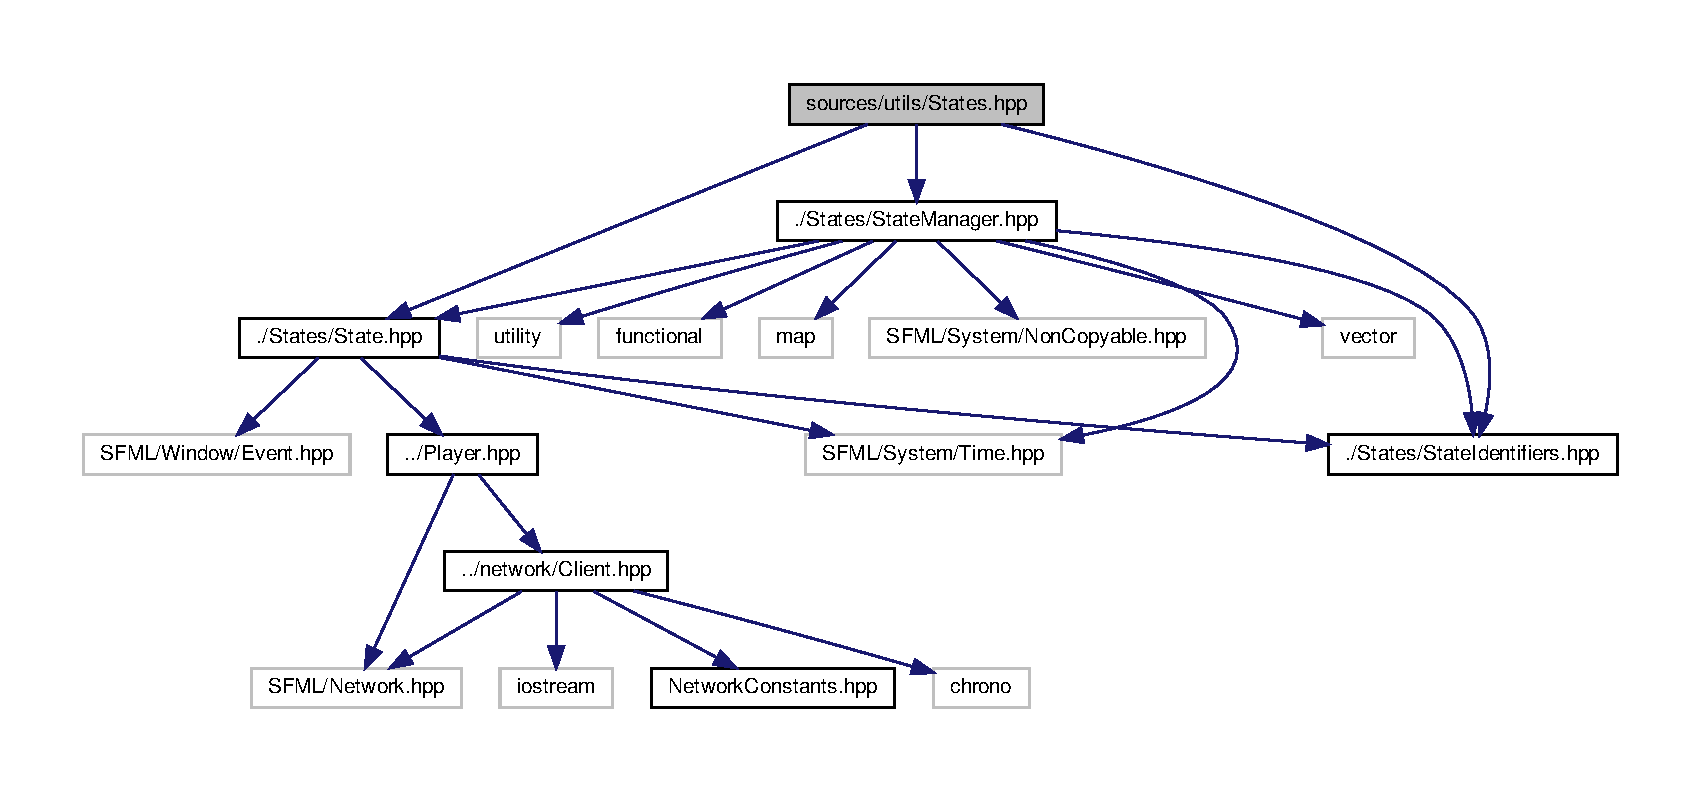
\includegraphics[width=350pt]{States_8hpp__incl}
\end{center}
\end{figure}
This graph shows which files directly or indirectly include this file\+:
\nopagebreak
\begin{figure}[H]
\begin{center}
\leavevmode
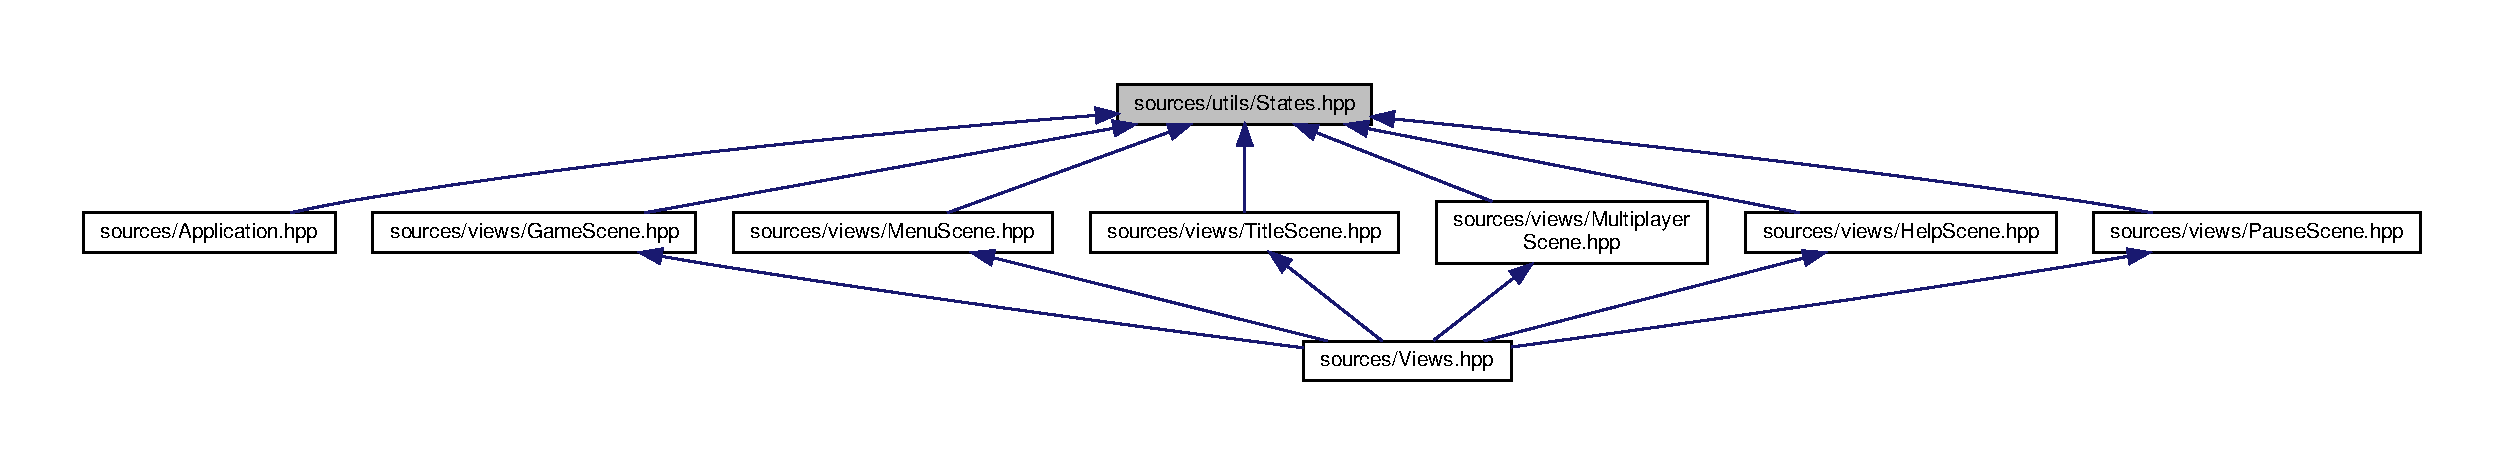
\includegraphics[width=350pt]{States_8hpp__dep__incl}
\end{center}
\end{figure}


\subsection{Detailed Description}
Compilation of paths to add State-\/related libraries. 

\begin{DoxyVersion}{Version}
0.\+1 
\end{DoxyVersion}
\begin{DoxyDate}{Date}
09/02/2020 
\end{DoxyDate}

\hypertarget{Views_8hpp}{}\section{sources/\+Views.hpp File Reference}
\label{Views_8hpp}\index{sources/\+Views.\+hpp@{sources/\+Views.\+hpp}}


Adds libraries needed to run.  


{\ttfamily \#include \char`\"{}./views/\+Game\+Scene.\+hpp\char`\"{}}\newline
{\ttfamily \#include \char`\"{}./views/\+Menu\+Scene.\+hpp\char`\"{}}\newline
{\ttfamily \#include \char`\"{}./views/\+Title\+Scene.\+hpp\char`\"{}}\newline
{\ttfamily \#include \char`\"{}./views/\+Multiplayer\+Scene.\+hpp\char`\"{}}\newline
{\ttfamily \#include \char`\"{}./views/\+Help\+Scene.\+hpp\char`\"{}}\newline
{\ttfamily \#include \char`\"{}./views/\+Pause\+Scene.\+hpp\char`\"{}}\newline
Include dependency graph for Views.\+hpp\+:
\nopagebreak
\begin{figure}[H]
\begin{center}
\leavevmode
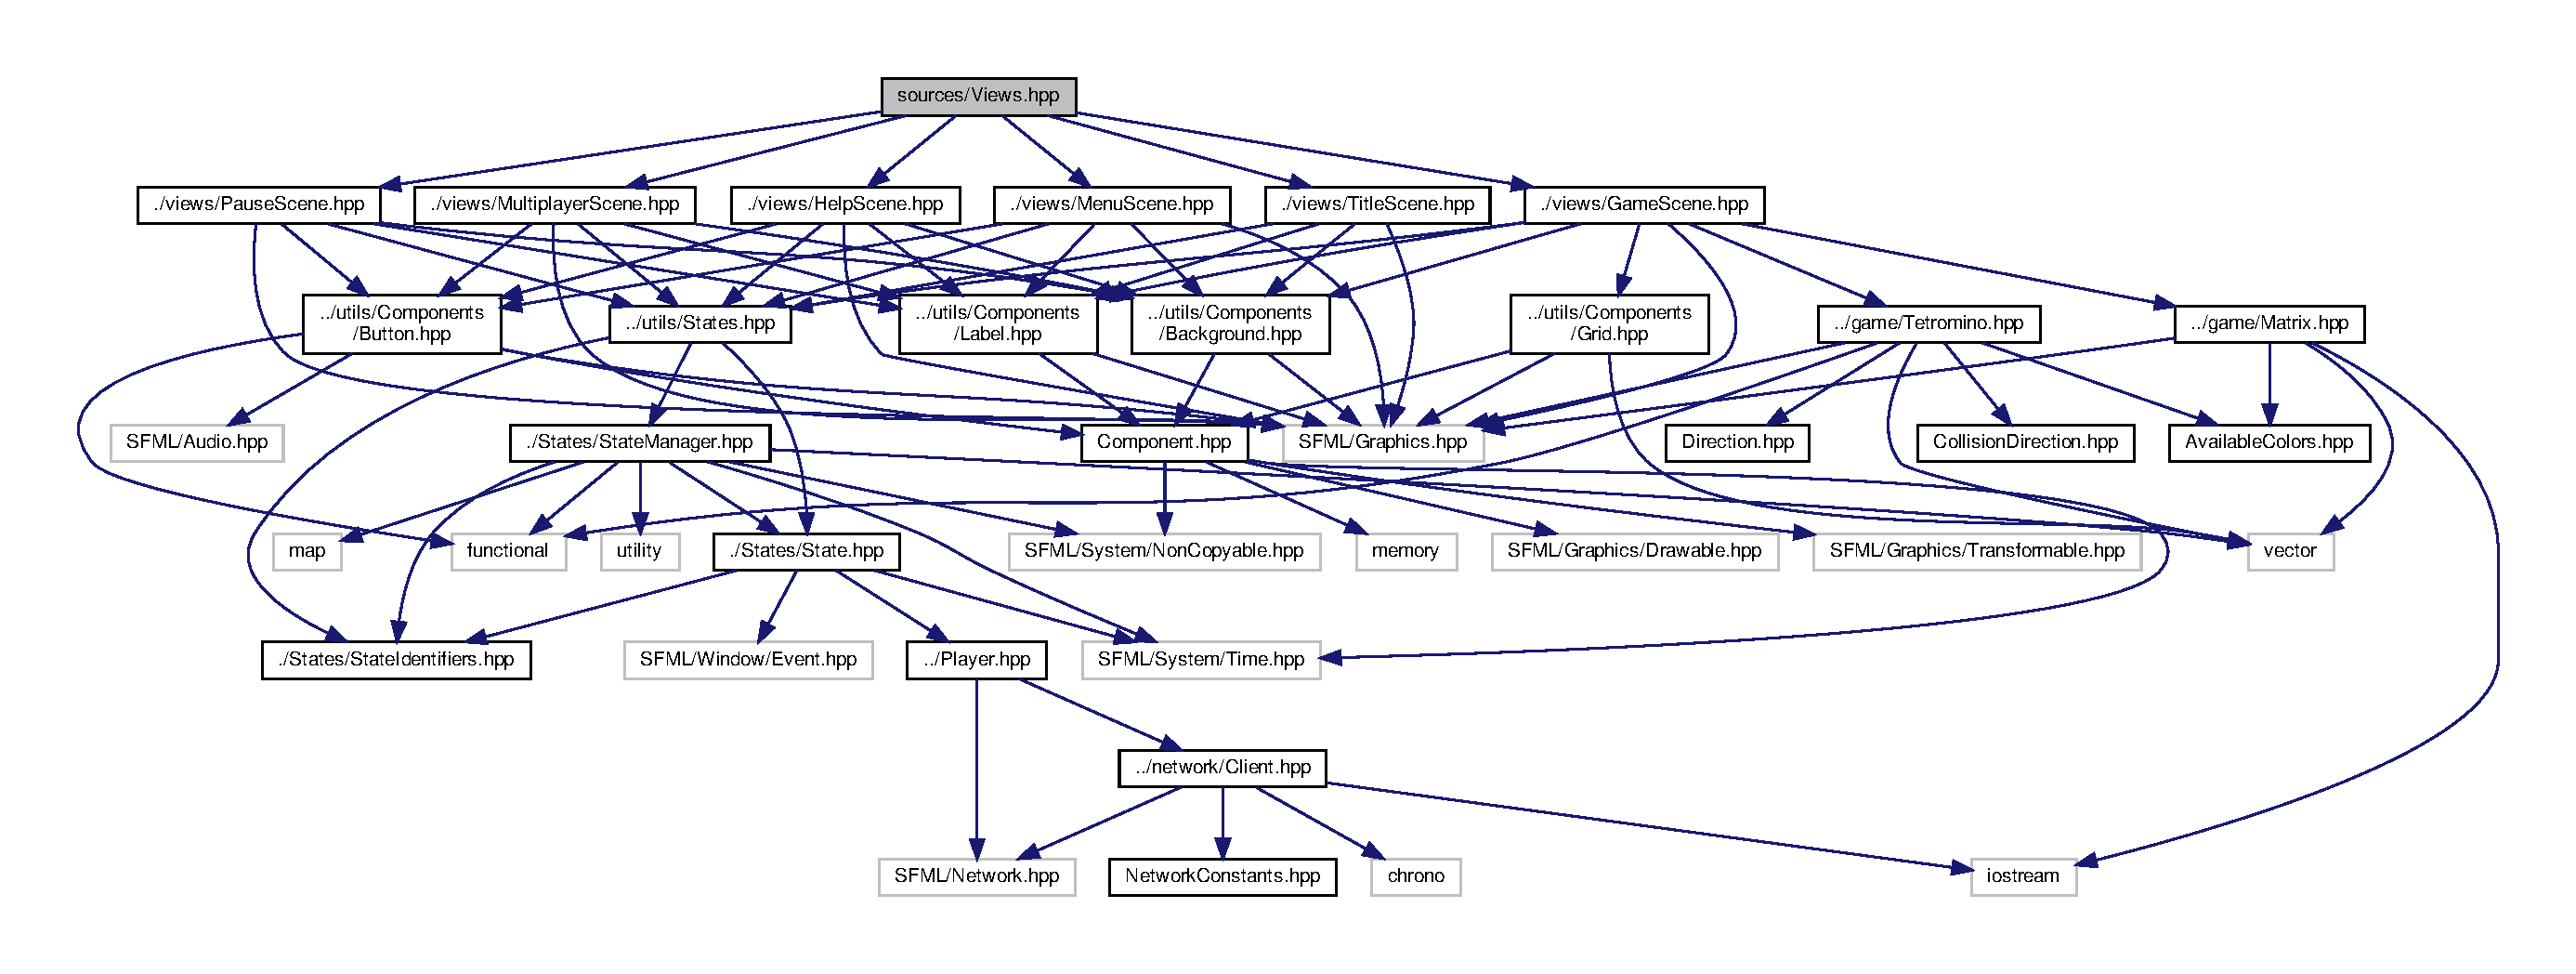
\includegraphics[width=350pt]{Views_8hpp__incl}
\end{center}
\end{figure}


\subsection{Detailed Description}
Adds libraries needed to run. 

\begin{DoxyVersion}{Version}
0.\+1 
\end{DoxyVersion}
\begin{DoxyDate}{Date}
09/11/2020 
\end{DoxyDate}

%--- End generated contents ---

% Index
\backmatter
\newpage
\phantomsection
\clearemptydoublepage
\addcontentsline{toc}{chapter}{Index}
\printindex

\end{document}
